%%%%%%%%%%%%%%%%%%%%%%%%%%%%%%%
%This is the article LaTeX template for RSC journals
%Copyright The Royal Society of Chemistry 2010
%%%%%%%%%%%%%%%%%%%%%%%%%%%%%%%


%\documentclass[8.5pt,twoside,twocolumn]{article}
\documentclass[11.5pt]{article}
\oddsidemargin -1.2cm
\evensidemargin -1.2cm
\textwidth 18cm
\headheight 1.0in
\topmargin -3.5cm
\textheight 22cm
\usepackage[super,sort&compress,comma]{natbib} 
\usepackage{mhchem}
\usepackage{times,mathptmx}
% \usepackage{times}
% feel free not to use mathptmx if it causes difficulties
\usepackage{sectsty}
\usepackage{balance} 
\usepackage{comment}
\usepackage{graphicx} %eps figures can be used instead
\usepackage{lastpage}
\usepackage{setspace}
\usepackage[format=plain,justification=raggedright,singlelinecheck=false,font=small,labelfont=bf,labelsep=space]{caption} 
\usepackage{fancyhdr}
\usepackage{multirow}
\usepackage{enumitem}
\usepackage{booktabs}
\usepackage{multicol}
\usepackage{array}
\newcolumntype{H}{>{\setbox0=\hbox\bgroup}c<{\egroup}@{}}
\pagestyle{fancy}

\newcommand{\bra}[2][0]
{\ifthenelse{\equal{#1}{0}}{\left\langle #2 \right|}
{\ifthenelse{\equal{#1}{1}}{\big\langle #2 \big|}
{\ifthenelse{\equal{#1}{2}}{\Big\langle #2 \Big|}
{\ifthenelse{\equal{#1}{3}}{\bigg\langle #2 \bigg|}
{\ifthenelse{\equal{#1}{4}}{\Bigg\langle #2 \Bigg|}
{Error}}}}}
}

% <#2|#3|#4>, #1 gives the size of the bracket
\newcommand{\bracket}[4][0]
{\ifthenelse{\equal{#1}{0}}{\left\langle #2 \middle| #3 \middle| #4 \right\rangle}
{\ifthenelse{\equal{#1}{1}}{\big\langle #2 \big| #3 \big| #4 \big\rangle}
{\ifthenelse{\equal{#1}{2}}{\Big\langle #2 \Big| #3 \Big| #4 \Big\rangle}
{\ifthenelse{\equal{#1}{3}}{\bigg\langle #2 \bigg| #3 \bigg| #4 \bigg\rangle}
{\ifthenelse{\equal{#1}{4}}{\Bigg\langle #2 \Bigg| #3 \Bigg| #4 \Bigg\rangle}
{Error}}}}}
}

% <#2|#3>, #1 gives the size of the bracket
\newcommand{\braket}[3][0]
{\ifthenelse{\equal{#1}{0}}{\left\langle #2 \middle| #3 \right\rangle}
{\ifthenelse{\equal{#1}{1}}{\big\langle #2 \big| #3 \big\rangle}
{\ifthenelse{\equal{#1}{2}}{\Big\langle #2 \Big| #3 \Big\rangle}
{\ifthenelse{\equal{#1}{3}}{\bigg\langle #2 \bigg| #3 \bigg\rangle}
{\ifthenelse{\equal{#1}{4}}{\Bigg\langle #2 \Bigg| #3 \Bigg\rangle}
{Error}}}}}
}

% |#2>, #1 gives the size of the bracket
\newcommand{\ket}[2][0]
{\ifthenelse{\equal{#1}{0}}{\left| #2 \right\rangle}
{\ifthenelse{\equal{#1}{1}}{\big| #2 \big\rangle}
{\ifthenelse{\equal{#1}{2}}{\Big| #2 \Big\rangle}
{\ifthenelse{\equal{#1}{3}}{\bigg| #2 \bigg\rangle}
{\ifthenelse{\equal{#1}{4}}{\Bigg| #2 \Bigg\rangle}
{Error}}}}}
}
\begin{document}
\thispagestyle{plain}
\fancypagestyle{plain}{
\fancyhead[L]{
\includegraphics[height=8pt]{headers/LH}}
\fancyhead[C]{\hspace{-1cm}
\includegraphics[height=20pt]{headers/CH}}
\fancyhead[R]{
\includegraphics[height=10pt]{headers/RH}\vspace{-0.2cm}}
\renewcommand{\headrulewidth}{1pt}}
\renewcommand{\thefootnote}{\fnsymbol{footnote}}
\renewcommand\footnoterule{\vspace*{1pt}% 
\hrule width 3.4in height 0.4pt \vspace*{5pt}} 
\setcounter{secnumdepth}{5}



\makeatletter 
\def\subsubsection{\@startsection{subsubsection}{3}{10pt}{-1.25ex plus -1ex minus -.1ex}{0ex plus 0ex}{\normalsize\bf}} 
\def\paragraph{\@startsection{paragraph}{4}{10pt}{-1.25ex plus -1ex minus -.1ex}{0ex plus 0ex}{\normalsize\textit}} 
\renewcommand\@biblabel[1]{#1}            
\renewcommand\@makefntext[1]% 
{\noindent\makebox[0pt][r]{\@thefnmark\,}#1}
\makeatother 
\renewcommand{\figurename}{\small{Fig.}~}
\sectionfont{\large}
\subsectionfont{\normalsize} 

\fancyfoot{}
\fancyfoot[LO,RE]{\vspace{-7pt}
\includegraphics[height=9pt]{headers/LF}}
\fancyfoot[CO]{\vspace{-7.2pt}\hspace{12.2cm}
\includegraphics{headers/RF}}
\fancyfoot[CE]{\vspace{-7.5pt}\hspace{-13.5cm}
\includegraphics{headers/RF}}
\fancyfoot[RO]{\footnotesize{\sffamily{1--\pageref{LastPage} ~\textbar  \hspace{2pt}\thepage}}}
\fancyfoot[LE]{\footnotesize{\sffamily{\thepage~\textbar\hspace{3.45cm} 1--\pageref{LastPage}}}}
\fancyhead{}
\renewcommand{\headrulewidth}{1pt} 
\renewcommand{\footrulewidth}{1pt}
\setlength{\arrayrulewidth}{1pt}
\setlength{\columnsep}{6.5mm}
\setlength\bibsep{1pt}

\noindent\LARGE{\textbf{Using Conventional Density Functionals to Simulate X-Ray Absorption Spectra: With Applications to Adenine and Thymine Photoabsorption Spectra}}
\vspace{0.6cm}

\noindent\large{\textbf{Wallace D. Derricotte, Francesco A. Evangelista.$^{\ast}$}}\vspace{0.5cm}
%Please note that \ast indicates the corresponding author(s) but no footnote text is required. 


\noindent\textit{\small{\textbf{Received Xth XXXXXXXXXX 20XX, Accepted Xth XXXXXXXXX 20XX\newline
First published on the web Xth XXXXXXXXXX 200X}}}

\noindent \textbf{\small{DOI: 10.1039/b000000x}}
\vspace{0.6cm}
%Please do not change this text.

\noindent \normalsize{Orthogonality Constrained Density Functional Theory (OCDFT) is used to compute excited states relevant to core-level spectroscopy, specifically the high lying excited states crucial to simulate near-edge x-ray absorption spectra (NEXAS). Density functional techniques that employ conventional exchange-correlation (XC) functionals routinely underestimate these excited states. This underestimation necessitates an artificial shift in the resulting spectra in order to make a comparison with experimental data. Here, we prove that OCDFT can accurately compute core excitation energies using conventional density functionals by assessing it's performance over a benchmarking test set of 40 core excitations. We utilize standard XC functionals (B3LYP, BLYP, PBE0), and compare these results with experimental data and time dependent density functional theory computations. We reveal the latent ability of OCDFT by simulating the gas-phase near-edge spectra of adenine and thymine. Our computations are consistent with previous NEXAS studies performed on these molecules and show dominant $\pi^*$ character mixed with definitive Rydberg transitions. The experimentally observed peak intensities are in excellent agreement with our calculated oscillator strengths, showing that OCDFT can accurately compute transition dipole moments.}
\vspace{0.5cm}

  \doublespacing
\section{Introduction}
The advent of synchrotron light sources created a strong resurgence of spectroscopy in the X-ray region. \cite{mcmillan_synchrotronproposed_1945} Near edge X-ray absorption spectroscopy (NEXAS) is a useful experimental technique to probe the local electronic and geometrical structure in a variety of molecular environments. It has been successfully applied to large biological systems, \cite{hua_refinement_2010} small molecules in the gas phase,\cite{contini_gas-phase_2001} organic thin-films,\cite{hahner_near_2006} and semiconducting materials.\cite{guo_electronic_2011} This wide range of applications is possible because synchrotron light sources can span an energy range that goes from a few electron volts (eVs) \cite{feneberg_synchrotron-based_2011} to hundreds of MeVs.\cite{nakazato_observation_1989} As NEXAS experiments are becoming increasingly more feasible, there is a growing need to develop accurate theoretical approaches to aid the interpretation of spectra.
The most dominant feature of this structure, the ``edge'', is composed of the excitations of core-electrons to unoccupied orbitals. In order for a method to properly replicate and analyze NEXAS spectra, it must demonstrate accuracy in describing core-electron excitations. 
Calculations of NEXAS spectra are challenging, and require computational methods that explicitly account for the excitations of core-level electrons, orbital relaxation effects, and electron correlation. \cite{coriani_coupled-cluster_2012} Several theoretical approaches have been adapted to compute core-valence excitations, including: scaled-opposite-spin configuration interaction singles with perturbative doubles [SOS-CIS(D)],\cite{asmuruf_calculation_2008} second-order algebraic digrammatic construction [ADC(2)],\cite{schirmer_beyond_1982,trofimov_efficient_1995} multiple scattering X$_\alpha$ methods, \cite{sheehy_correlation_1989} a maximum overlap $\Delta$SCF approach, \cite{besley_self-consistent-field_2009} transition potential theory,\cite{triguero_calculations_1998} coupled-cluster response theory, \cite{coriani_coupled-cluster_2012} and time-dependent density functional theory (TDDFT).\cite{stener_time_2003} Among these methods TDDFT is a very attractive option because of its reduced computational cost and ability to calculate multiple excited states.

Within the density functional theory framework, TDDFT is regarded as the method of choice to treat electronic excited states because it is a rigorous extension of the ground-state formalism.\cite{runge_density-functional_1984} When applied in conjunction with frequency-independent exchange-correlation potentials, TDDFT yields accurate excitation energies for low-lying excited states. For example, the TDDFT benchmark study of Silva-Junior and co-workers\cite{silva-junior_benchmarks_2008} on 28 organic molecules, showed that singlet and triplet excitation energies can be calculated with a mean average error (MAE) of 0.27 eV and 0.44 eV, respectively. However, Besley et al.\cite{besley_self-consistent-field_2009} showed that TDDFT core excitations computed with conventional exchange-correlation functionals grossly underestimate experimental results, yielding a MAE of 20.2 eV.  Given the difficulties encountered by TDDFT in computing charge-transfer excited states\cite{dreuw_failure_2004} and the self interaction error that afflicts traditional density functionals, this failure is to be expected.
Work by Peach et al. \cite{peach_excitation_2008} suggests that there is a direct correlation between the accuracy of TDDFT and the degree of spatial overlap ($\Lambda$) between the occupied and virtual orbitals involved in the excitation. Low orbital overlap is a characteristic feature of both charge transfer excitations and core excitations, with the relationship between accuracy and orbital overlap being persistent through core excitations as well. \cite{besley_time-dependent_2009}
The inaccuracy of TDDFT for excitations with low values of $\Lambda$ has been attributed to the incorrect asymptotic behavior of the exchange-correlation potential and self-interaction error.

In the case of core-valence excitations, quantitative agreement with experiment is only attained by using a self-interaction correction (SIC),\cite{tu_core_2007} or range separated hybrid functionals in which the amount of long and short range Hartree--Fock exchange is reparametrized.\cite{besley_time-dependent_2009, nakata_time-dependent_2006} This is often the limiting factor for studying the edge structure of many chemical systems since the optimal amount of Hartree--Fock exchange varies with each unique system being studied.\cite{capano_role_2013,besley_time-dependent_2007,besley_time-dependent_2010} A method that can systematically produce accurate core-excitation energies with traditional hybrid density functionals is highly desirable. The maximum overlap method (MOM) \cite{besley_self-consistent-field_2009} combined with a $\Delta$SCF treatment of core-valence excitations is able to obtain highly accurate excitation energies using conventional functionals. However, this procedure is not guaranteed to avoid the problem of variational collapse---albeit MOM ameliorates the difficulties encountered by a straightforward $\Delta$SCF procedure---and has not been generalized to multiple excited states of the same symmetry.

Orthogonality constrained density functional theory (OCDFT)\cite{evangelista_orthogonality_2013}  is a variational, time-independent formulation of excited state DFT that maintains the favorable accuracy/cost ratio of traditional DFT. It builds upon previous successful efforts to formulate time-independent excited state DFT, such as: the $\Delta$SCF procedure, \cite{kowalczyk_assessment_2011,ziegler_calculation_1977} constrained DFT,\cite{wu_constrained_2006} stationary state DFT, \cite{gorling_density-functional_1999} self-consistent field constricted variational density functional theory (SCF-CV-DFT) , \cite{ziegler_relation_2009,ziegler_application_2011,krykunov_self-consistent_2013,ziegler_implementation_2012} excited state ensemble DFT \cite{theophilou_energy_1979,fritsche_generalized_1986,gross_rayleigh-ritz_1988,gross_density-functional_1988} variational time independent DFT (TI-DFT) \cite{levy_variational_1999,nagy_variational_2001} Benchmark computations show that valence excitation energies computed with OCDFT have error metrics comparable to that of TDDFT.  In addition, OCDFT has the ability to accurately compute charge transfer excitation energies regardless of the amount of Hartree-Fock exchange present in the exchange-correlation functional.

This work extends the applicability of OCDFT to the calculation of X-ray  absorption near-edge structure by introducing two new developments.
First, we formulate an OCDFT algorithm that can be used to compute core-valence excitation energies.  This new method is assessed over a test set that includes 13 molecules with 40 unique core-electron excitations.
Second, we discuss one approach to extend OCDFT to multiple excited states of the same symmetry.
We demonstrate the potential of this new method with computations of the gas-phase near-edge spectra of adenine and thymine.


\section{Theory}
In this section we provide a brief summary of orthogonality constrained density functional theory along with the necessary extension to multiple excited states (for the full details of the OCDFT derivation we refer the reader to Ref.\citenum{evangelista_orthogonality_2013}) OCDFT is a time-independent variational formulation of DFT that builds upon the approach developed by Ayers, Levy, and Nagy.\cite{ayers_time-independent_2012} OCDFT supplements this formulation by implementing a Kohn-Sham (KS) scheme in which the KS energy functional is augmented with an orthogonality constraint between the ground state and excited state wavefunctions
\begin{align}
\braket[1]{\Phi^{(\text{1})}}{\Phi} &= 0 ,
\end{align} 
where $\Phi^{(1)}$ is a Slater determinant wavefunction representing the first excited state built in the KS spin orbital basis \{$\phi_i^{(1)}$\} and $\Phi$ is the ground state determinant. Imposing this constraint  introduces an explicit hole orbital ($\phi^{(1)}_h$) and particle orbital ($\phi^{(1)}_p$) for the excited state. Where $\phi^{(1)}_h$ represents the orbital in the occupied space that the electron was promoted from and $\phi^{(1)}_p$ represents the orbital in the virtual space that the electron now occupies in the excited configuration. These orbitals naturally satisfy the following conditions 
\begin{align}
\hat{Q}\phi_h^{(1)} &= 0 , \\
\hat{P}\phi_p^{(1)} &= 0 ,
\end{align}
where $\hat{P}$ and $\hat{Q}$ are projections onto the occupied and virtual space of $|\Phi \rangle$ respectively. By restricting the space spanned by $\phi^{(1)}_h$ and $\phi^{(1)}_p$, equations 2 and 3 are enforcing the fact that an electron can not be promoted from a virtual orbital or promoted to an occupied orbital. The projection operators are designed to span over the entire occupied and virtual space by taking the total summation of the outer products of every orbital contained in the set.
\begin{align}
\hat{P} &= \sum_i^{\text{occ}} |\phi_i\rangle \langle \phi_i| , \\
\hat{Q} &= \sum_a^{\text{vir}} |\phi_a\rangle \langle \phi_a| .
\end{align}
The orthogonality condition is enforced explicitly for the hole orbital through the use of Lagrange multipliers. The resulting Lagrangian minimizes the excited state energy with respect to the orthogonality constraints
\begin{align}
\nonumber \mathcal{L}^{(1)}[\{\phi_i^{(1)}\}, \phi^{(1)}_{\text{h}}] = &E^{(1)}_{\text{KS}}[\{\phi_i^{(1)}\}] + \sum_a^{\text{vir}} \lambda_a \langle \phi^{(1)}_{\text{h}}|\phi_a\rangle  \\ 
&- \sum_{pq} \epsilon^{(1)}_{pq} (\langle \phi^{(1)}_{p}|\phi_q^{(1)}\rangle - \delta_{pq}) ,
\end{align}
The second term of the Lagrangian explicitly enforces the orthogonality constraint between the hole orbital and the ground state virtual set that was introduced in equation 2, while the last term enforces the general orbital orthogonality condition between the excited state orbitals. E$^{(1)}_{\text{KS}}[\{\phi_i^{(1)}\}]$ is the standard KS energy functional for the excited state. Setting the variation of the Lagrangian with respect to $\{\phi^{(1)}_i\}$ and $\phi^{(1)}_h$ to zero results in a set of stationary conditions that lead to the following eigenvalue equation:
\begin{align}
\hat{P}(1-\hat{Q_s}) \hat{f} |\phi_h^{(1)}\rangle &= \epsilon_h |\phi_h^{(1)}\rangle ,
\end{align}
where $\hat{Q}_s$ is the projection onto the orbitals that are in the virtual space but not involved in the excitation, we refer to such orbitals as ``spectators''. 
%and  $\epsilon_h^{(1)}$ is the energy eigenvalue of the KS Hamiltonian with respect to the hole orbital basis $\{\phi_h^{(1)}\}$.
These projection operators have an intuitive identity that  for any excited state $k$, $\hat{P}$ and $\hat{Q}$  must sum to unity.
\begin{align}
\hat{P}^{(k)} + \hat{Q}^{(k)} = 1 .
\end{align}
\begin{figure}
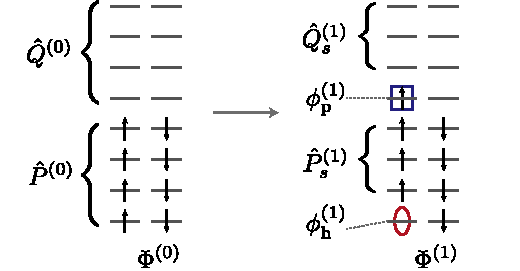
\includegraphics[scale=0.35]{Figure1.pdf}
\caption{Visual representation of the space spanned by all projection operators for the ground state determinant $|\Phi\rangle$ and the excited state determinant $|\Phi^{(1)}\rangle$. Notice that the hole orbital comes from the space spanned by $\hat{P}$ and that the particle orbital comes from the space spanned by  $\hat{Q}$, this is a direct result of Equations 2 and 3.}
\end{figure}
This identity reveals the physical significance of the $1 - \hat{Q}_s$ operator that appears in equation 7, as it can be interpreted as the projection onto the entire excitation space for a given state, a visual representation of this is shown in Figure 1. The algorithm detailed in equation 7 constrains the hole orbital basis, thus we refer to it as the constrained hole (CH) algorithm. It is possible to extend this formulation to multiple excited states by simply removing the hole belonging to the previous excited state from the spectator space
\begin{align}
%\notag (1-\hat{Q}) (1 - \hat{Q}_s)\hat{f} |\phi_{\text{h}}^{\text{(1)}}\rangle &= \epsilon^{\text{(1)}}_{\text{h}} |\phi_{\text{h}}^{\text{(1)}}\rangle \\
%\notag (1-\hat{Q}) (1 - \hat{Q}_s - (\hat{P}^{(1)}_{\text{h}}))\hat{f} |\phi_{\text{h}}^{\text{(2)}}\rangle &= \epsilon^{\text{(2)}}_{\text{h}} |\phi_{\text{h}}^{\text{(2)}}\rangle \\ 
%\notag (1-\hat{Q}) (1 - \hat{Q}_s - (\hat{P}^{(1)}_{\text{h}} + \hat{P}^{(2)}_{\text{h}}))\hat{f} |\phi_{\text{h}}^{\text{(3)}}\rangle &= \epsilon^{\text{(3)}}_{\text{h}} |\phi_{\text{h}}^{\text{(3)}}\rangle\\
%\notag \vdots\\
\hat{P}[1 - \hat{Q}_s - (\hat{P}^{(1)}_{\text{h}} + \hat{P}^{(2)}_{\text{h}} + ... +\hat{P}^{\text{(k-1)}}_{\text{h}})]\hat{f} |\phi_{\text{h}}^{\text{(k)}}\rangle &= \epsilon^{\text{(k)}}_{\text{h}} |\phi_{\text{h}}^{\text{(k)}}\rangle .
\end{align}
Using this method extends the CH algorithm to allow the calculation of any excited state ``$k$''. We refer to this as the multi-constrained hole projection (MCHP) algorithm. It is important to note here that the ordering of the energy eigenvalues is not arbitrary, they are ordered by increasing orbital energy
\begin{align}
\epsilon^{\text{(1)}}_{\text{h}} \le \epsilon^{\text{(2)}}_{\text{h}} \le \epsilon^{\text{(3)}}_{\text{h}} \le ... \le \epsilon^{\text{(k)}}_{\text{h}} .
\end{align}
Because of this, in order for the MCHP algorithm to obtain the energy for the $k^{\text{th}}$ excited state, it must first project out all holes related to excited states 1 $\rightarrow$ $(k-1)$.

\section{Computational Details}
OCDFT was used to compute 40 unique core-excitations from a test set of 13 molecules. Its accuracy was assessed by comparing it to experimental data from gas-phase NEXAS experiments.\cite{puttner_vibrationally_1999,remmers_high-resolution_1992,chen_k-shell_1989,tronc_nitrogen_1980,tronc_carbon_1979,francis_studies_1994,adachi_vibronic_1999,hitchcock_k-shell_1979,domke_carbon_1990,nayandin_angle-resolved_2001,bodeur_single-and_1990} Excitations from 1s orbitals are considered for all multi-electron atoms in each molecule, in addition to excitations from 2p orbitals for second row elements. All structures were optimized using the Karlsruhe triple zeta valence polarization (def2-TZVP) basis set\cite{weigend_balanced_2005,weigend_accurate_2006} available in the \textsc{psi4} \textit{ab initio} quantum chemistry package.\cite{turney_psi4:_2012} Optimized geometries and excitation energies were computed consistently using the same functional.
\\ \\
The inclusion of scalar relativistic effects are a common practice when studying excitations of core electrons.\cite{maganas_l-edge_2014,debeer_george_calibration_2010,bauer_herfd-xas_2014,ankudinov_sensitivity_2002} It was rigorously proven by Levy \cite{levy_excitation_1995} that the excitation energy, $\omega$, can be expressed in terms of ground state KS orbital energies ($\epsilon$) in the following way
\begin{align}
\omega = \epsilon_{\text{p}} - \epsilon_{\text{h}} + \Delta \nu_{\text{xc}} 
\end{align}
Where the p and h subscripts denote the particle and hole orbitals involved in the excitation and $\Delta \nu_{\text{xc}} $ is the potential difference between the ground state and the excited state. Work by Desclaux et al. \cite{desclaux_relativistic_1971} shows that the largest orbital effect when solving the relativistic hartree-fock equations is the contraction of the 1s orbital, this contraction ($\gamma^{\text{1s}}$) can be approximated by observing the energy reduction of the orbital between a nonrelativistic (NR) and relativistic (R) calculation as shown in Equation 12
\begin{align}
\gamma^{\text{1s}} = \epsilon_{\text{1s}}^{\text{R}} \  - \epsilon_{\text{1s}}^{\text{NR}}.
\end{align}
The relativistic orbital energies were obtained using the Douglass-Kroll Hess (DKH) Hamiltonian \cite{douglas_quantum_1973,hess_applicability_1985, hess_relativistic_1986}, and then the subsequent $\gamma^{\text{1s}}$ is applied directly to the excitation energy
\begin{align}
\omega = \epsilon_{\text{p}} - \epsilon_{\text{h}} + \Delta \nu_{\text{xc}} + \gamma^{\text{1s}} .
\end{align}
The relativistic correction for first row 1s core orbitals are negligibly small (C, N, and O 1s contractions are approximately 0.1, 0.2, and 0.3 eV respectively). Relativistic corrections for the 1s orbitals of the second row nuclei ranged from 3.8 eV (Si) to 10.1 eV (Cl). Excitations from 2p orbitals of second row elements are negligible (max 0.05 eV) and were not applied to the final results. \\
The treatment of core-excited states in highly symmetric molecules presents a unique challenge for conventional DFT functionals that are based on the local density approximation (LDA). The existence of symmetry equivalent atoms becomes problematic for both pure and hybrid functionals due to the approximate treatment of exchange and correlation which introduces a self-interaction error.\cite{lundberg_quantifying_2005} A classic example of this problem is the dissociation of the H$_2^+$ ion, where at large distances, standard functionals artificially stabilize a state of delocalized density because of the decrease in self-interaction.\cite{bally_incorrect_1997} The interaction between core excitations on equivalent atomic centers is weak, and thus these excitations are inherently local. To obtain a state where the core hole is localized, we utilize a wavefunction with broken spatial and spin symmetry for all molecules with symmetry equivalent atoms in the test set (N$_2$, C$_2$H$_2$, and Cl$_2$).
\section{Results and Discussion}
The MAEs of OCDFT over the abridged test set are shown in Table \ref{table:OverallPerformance}, considering 12 unique basis set and functional combinations. A direct comparison of the accuracy of OCDFT and TDDFT compared to experimental core-excitation energies are shown in Figure \ref{figure:Hist}. A breakdown of individual excitations computed with OCDFT and TDDFT are compared to their experimental assignments in Tables \ref{table:FirstRow} and \ref{table:SecondRow}. Table \ref{table:FirstRow} displays excitations from first row atoms, while Table \ref{table:SecondRow} shows excitations from second row atoms. We observe a distinct relationship between the amount of hole/particle orbital overlap and the accuracy of the computations, this relationship is explained in Section 4.3 and further analyzed in Figure \ref{figure:scatter}. Finally we close by computing the NEXAS spectra of two nucleobases, adenine and thymine. The nitrgen, carbon, and oxygen edges for Thymine can be found in Figure \ref{figure:Thymine} while the carbon and nitrogen edges of Adenine are found in Figure \ref{figure:Adenine}. Spectra resulting from inner-shell ionizations are commonly referred to as K, L, or M edges depending on which core-shell is involved in the excitation. This nomenclature is simply derived from the Barkla labeling scheme for x-ray series, and we will routinely employ it to refer to specific spectra.
\subsection{Overall Performance}
The performance of OCDFT on the full test set of first and second row core excitations with different functionals and basis sets is shown in Table \ref{table:OverallPerformance}. The data shows no dramatic difference in the accuracy of OCDFT regardless of the amount of Hartree-Fock (HF) exchange present in the functional. Even the BLYP functional, shows comparable accuracy to its hybrid counterparts. BLYP often outperforms PBE0 and yields similar MAEs as B3LYP across all basis sets. The Karlsruhe family of basis sets give the most accurate result, while the correlation consistent (cc) basis sets also perform well, however are slightly less accurate than the Karlsruhe basis sets.
\begin{table}[!ht]
    \begin{tabular}{l@{\hskip 0.5in}lll}
    \hline
    \hline
Basis Set & \multicolumn{3}{c}{Mean Absolute Error (eV)}  \\
\hline
& BLYP & B3LYP & PBE0\\
def2-TZVP & 1.0 & 1.0 & 0.9 \\
def2-QZVP & 1.0 & 1.0 & 1.4 \\
cc-pCVTZ & 1.3 & 1.3 & 1.6 \\
cc-pCVQZ & 1.5 & 1.5 & 1.7 \\
\end{tabular}
    \caption{Mean absolute error in the core-excited states calculated using OCDFT on a test set of 35 different core excited states from 13 different molecules.}
    \label{table:OverallPerformance}
\end{table}
\\ \\ 
The average error of OCDFT is commensurate to wavefunction methods that have been used to treat core-excited states. Asmuruf and Besley\cite{asmuruf_calculation_2008} reported an average error of 1.2 eV for SOS-CIS(D) applied to a set of excitations similar to the ones used in the present study. While Coriani et al.\cite{coriani_coupled-cluster_2012} reported errors of less than 0.9 eV when applying coupled cluster response theory to a set of carbon, nitrogen, and neon core excitations. These methods are still not as accurate as computations done on valence excitations, which were shown to have a mean average error of 0.14 eV in a recent extensive TD-DFT benchmark when using conventional CI or DFT methods. \cite{jacquemin_extensive_2009} 
\\ \\
A full comparison of the accuracy of OCDFT and TDDFT in tandem with the B3LYP functional and def2-QZVP basis applied to first row and second row core excitations is shown in Fig. \ref{figure:Hist}. OCDFT performs very well, peaking at an error close to zero and its largest error being $-$3.7 eVs. On the contrary, TDDFT performs rather poorly, peaking at an error close to $-$15 eVs and its largest error being $-$53.6 eVs. To understand why OCDFT outperforms TDDFT, we will compare the singlet excitation energy expression of CIS to TDDFT. Similar analyses have been done on variational DFT \cite{ziegler_implementation_2012} and TDDFT \cite{casida_charge-transfer_2000}. The excitation energy for TDDFT differs from the CIS excitation energy by a term that includes nonlocal integrals that rely on both the hole and particle functions simulataneously
\begin{align}
 \nonumber \omega^{\text{TDDFT}}_s = \ &\omega^{\text{CIS}}_s + (1 - a) [J_{\text{ph}} - J_{\text{hh}}] \\ &+ (1 - a) [\nu_{\text{p}}^x - \nu_{\text{h}}^x] ,
\end{align}
where $\nu_i^x$ is the exchange potential and $a$ is a parameter that weights the relative amount of DFT and HF exchange. The nonlocal $\hat{J}_{\text{ph}}$ coulomb repulsion integral is problematic and leads to a poor description of the coulombic attraction that exists between a positively charged hole and a negatively charged particle. Thus, it can not naturally describe core excitations, and relies instead on the varying of the $a$ parameter to increase accuracy. The improved performance of OCDFT for core excited states is largely due to the local nature of the integrals involved. The excitation energy for OCDFT differs from CIS by a term that is composed of integrals that are localized on either the hole or the particle, which guarantees it will be exact for low orbital overlap systems
\begin{align}
\nonumber \omega^{\text{OCDFT}}_s = \ &\omega^{\text{CIS}}_s + (1 - a) [\nu_{\text{p}}^x - \nu_{\text{h}}^x + \frac{1}{2} J_{\text{pp}} - \frac{1}{2} J_{\text{hh}} \\
&+ \frac{1}{2} (\text{hh}|\hat{f}_x|\text{hh}) +\frac{1}{2} (\text{pp}|\hat{f}_x|\text{pp})] ,
\end{align}
where (ii$|\hat{f}_x|$ii) = $\int |\phi_{\text{i}}|^2\ \hat{f}_x\  |\phi_{\text{i}}|^2 \ d\tau$ are the exchange kernel integrals. The local nature of the integrals in this term provide a better approximation to exact exchange. This is a direct consequence of the orthogonality condition imposed between the ground and excited states, resulting in a term that is much more adept at handling systems with low orbital overlap.
\begin{figure}[!ht]
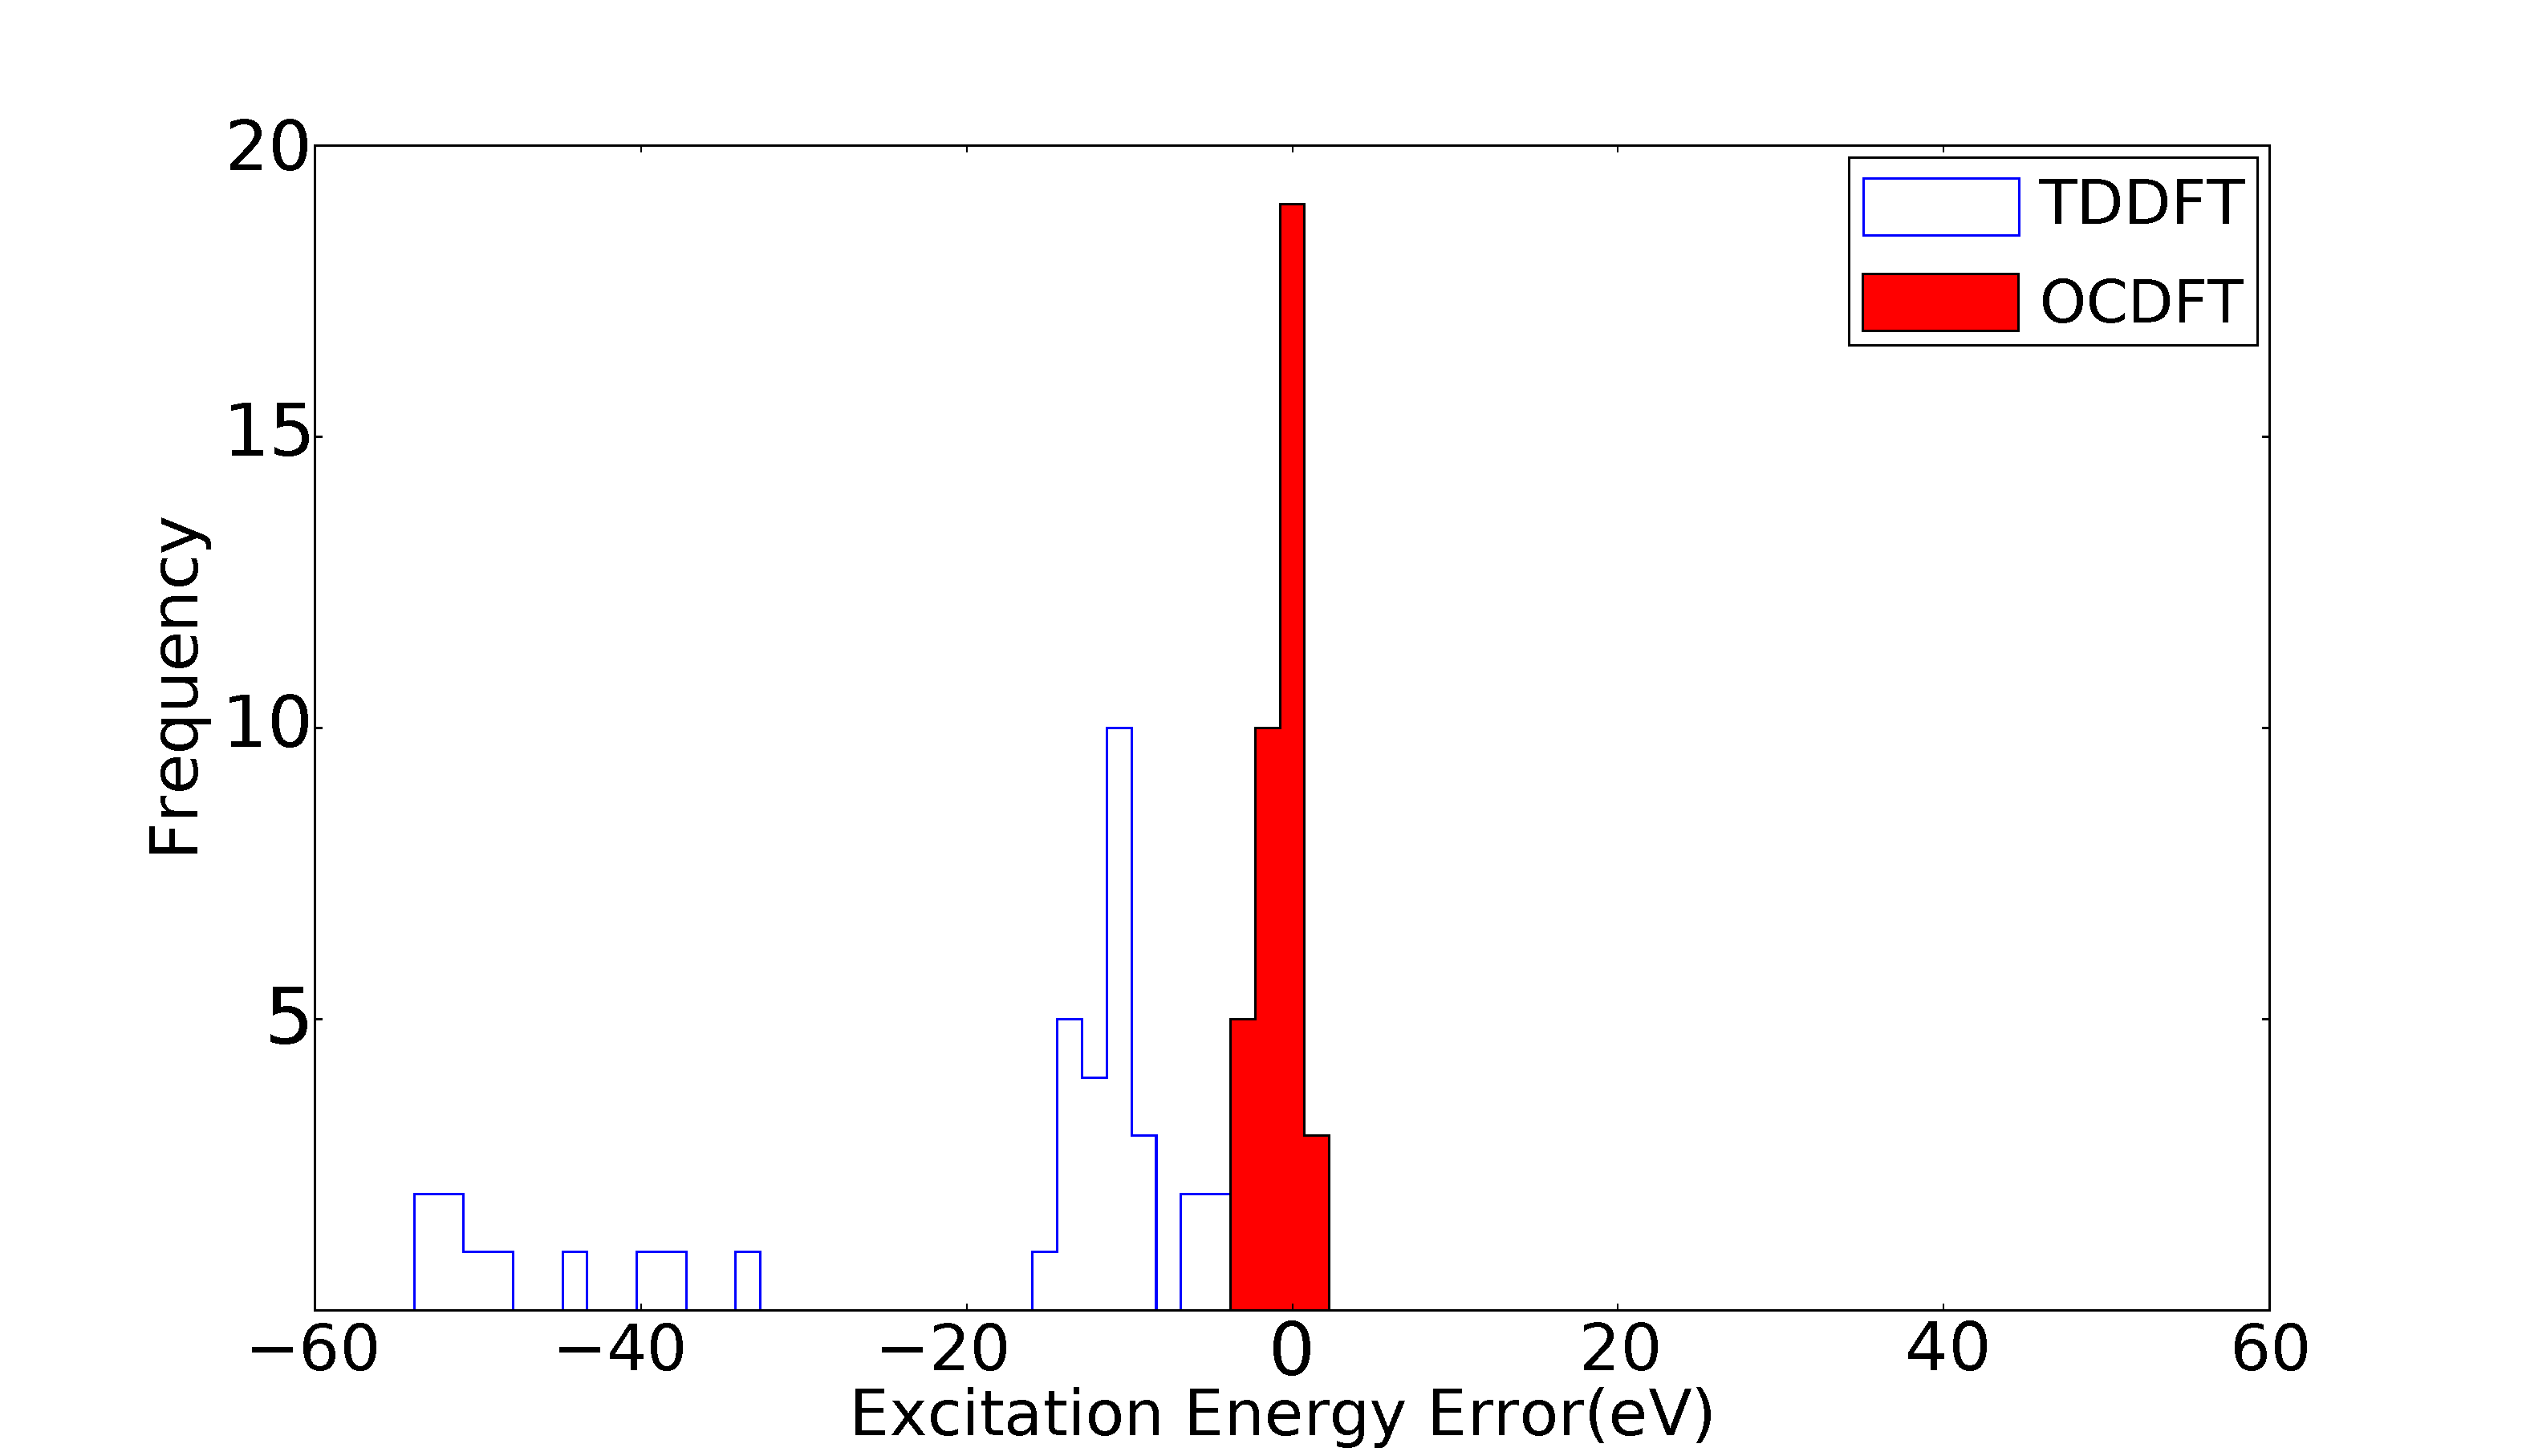
\includegraphics[scale=0.17]{TDDFT_OCDFT_histogram.pdf}
\caption{Histogram showing the distribution of the error in the computed core excited states. All calculations were done using the B3LYP functional and the def2-QZVP basis set. The red filled bar is OCDFT while the empty blue bar is TDDFT.}
\label{figure:Hist}
\end{figure}
\\ \\
Fig. \ref{figure:Hist} hints at a specific difficulty of conventional TDDFT. Notice the gap, roughly 15 eV wide, that exists between the two clusters of TDDFT data. This gap exists because TDDFT becomes sharply more inaccurate when dealing with second row core excitations, even when relativistic corrections are included. All of the TDDFT errors that are higher in magnitude than -20 eVs can be attributed to core excitations involving 1s orbitals located on second row nuclei. This dramatic drop in accuracy suggests that it is helpful to consider first row and second row core excitations seaparately to highlight the distinctive challenges that arise in each case.
\subsection{First-Row Core Excitations}
\noindent Table \ref{table:FirstRow} shows valence and Rydberg excited states in which the core orbital is localized on the 1s orbital of a first row element (C, N, or O). Excitation energies were calculated using TDDFT and OCDFT in tandem with the B3LYP functional and basis sets of quadruple zeta quality. TDDFT produces a mean absolute error of 11.6 eVs compared to experiment, and as discussed earlier, this is consistent with previous studies that used TDDFT with a conventional hybrid functional.\cite{besley_self-consistent-field_2009} OCDFT calculations under the same conditions yield a mean absolute error of 0.4 eV. To put this error into perspective, it can be compared to the performance of TDDFT with the BH$^{0.58}$LYP functional,\cite{besley_time-dependent_2009} a reparameterization of the BHLYP functional that has been augmented to include 58\% HF exchange, 39\% B88 exchange, and 8\% Slater exchange. When applied to a test set similar to those in Figure \ref{table:FirstRow}, BH$^{0.58}$LYP yielded a mean average error of 0.8 eVs. A comparable level of accuracy was achieved by OCDFT without altering the inherent amount of HF exchange present in the functional.
\\ \\
It is customary to remedy the deficiency of TDDFT by shifting the position of the computed spectra by an amount that minimizes the difference between the computational and experimental peak features. In the case of the first row elements, this would imply shifting the TDDFT spectra by about 10 eV and using an even larger shift when dealing with heavier atoms. For example, a study done by DeBeer, Petrenko, and Neese\cite{debeer_george_prediction_2008} showed that it is necessary shift the TDDFT Fe near-edge spectra of different iron complexes by 171.3 eV in order to correct the spectra. For OCDFT the computed excitation energies are in good agreement with experiment, making these corrective shifts unnecessary.
\\ \\ 
\begin{table*}[t]
    \centering
    \begin{tabular}{lll@{\hskip 0.6in}llHH}
    \hline
    \hline
     Molecule & Excitation                     & Exp.&TDDFT  &OCDFT          &     \\
     \hline
    ~         & ~                              &   & & & TDDFT    & OCDFT \\
    \multirow{4}{*}{CO}        & C 1s $\rightarrow$ $\pi^*$     & 287.4 & -11.3     & -0.8  & -10.9    & \ 0.9   \\
             & C 1s $\rightarrow$ 3s          & 292.4 & -10.5     & \ 0.9   & -10.8    & \ 1.2   \\
             & O 1s $\rightarrow$  $\pi^*$    & 534.2 & -13.4     & -1.2  & -14.4    & -1.4   \\
             & O 1s $\rightarrow$ 3s          & 538.9 & -13.0     & \ 0.2 \vspace{2mm}   & -13.9    & \ 0.3 \\ 
    \multirow{4}{*}{H$_2$CO }     & C 1s $\rightarrow$ $\pi^*$     & 286.0   & -10.7     & -0.6  & -10.7    & -0.8   \\
    ~         & C 1s $\rightarrow$ 3s          & 290.2 & -10.7     & -0.2   & -10.7    & -0.3   \\
    ~         & O 1s $\rightarrow$ 3s          & 535.4 & -14.1     & -0.6   & -14.1    & -0.7   \\
    ~         & O 1s $\rightarrow$  $\pi^*$    & 530.8 & -14.0    & -0.8 \vspace{2mm}   & -14.1    & -1.1  \\
    \multirow{6}{*}{N$_2$O$^{\dagger}$}    &O 1s  $\rightarrow$ $\pi^*$ &  534.8 & -14.3 &  -1.0 & -14.3 & -1.3 \\
    ~         &O 1s  $\rightarrow$ 3s &  536.7 & -13.6 &  -0.4 & -13.6 & -0.6 \\
    ~         & N$_\text{c}$ 1s $\rightarrow$ 3s      & 407.5 & -12.1     & \ 0.6   & -12.6    & \ 0.6   \\
    ~         & N$_\text{t}$ 1s $\rightarrow$ $\pi^*$ & 401.1 & -12.2     & -0.9  & -14.6    & \ 2.5   \\
    ~         & N$_\text{t}$ 1s $\rightarrow$ 3s      & 404.0   & -11.5    & -0.4  \vspace{2mm} & -11.0    & -0.5  \\
    \multirow{3}{*}{N$_2$}         &N 1s  $\rightarrow$ $\pi^*$ & 401.0 & -12.4 & -0.9 & -12.4 & -1.1 \\
    ~         & N 1s  $\rightarrow$ 3s & 406.2 & -8.5 & 1.7 \vspace{2mm} & -7.2 & \ 2.7\\ 
    \multirow{4}{*}{HCN}       & C 1s $\rightarrow$ $\pi^*$     & 286.4 & -10.6     & -0.5  & -10.6    & -0.7  \\
    ~         & C 1s $\rightarrow$ 3s          & 289.1 & -9.9      & -0.1   & -9.9    & -0.3  \\
    ~         & N 1s $\rightarrow$  $\pi^*$    & 399.7 & -12.0     & -0.8  & -12.0    & -1.0  \\
    ~         & N 1s $\rightarrow$ 3s          & 401.8 & -10.4      & \ 0.2 \vspace{2mm}   & -10.4    & \ 0.0  \\
    \multirow{2}{*}{CH$_4$}      & C 1s $\rightarrow$ 3p          & 288.0   & -10.1      & \ 0.1   & -10.1    & \ 0.0   \\
    ~         & C 1s $\rightarrow$ 3s          & 287.1 & -10.8    & -0.5 \vspace{2mm}  & -10.8     & -0.6 \\ 
        \multirow{2}{*}{C$_2$H$_2$}      & C 1s $\rightarrow$ $\pi^*$           & 285.8   & -10.5      & -0.1   & -10.4   & -0.7  \\
    ~         & C 1s $\rightarrow$ 3s            & 287.7 & -9.1 & -0.6 \vspace{2mm}  & -8.9    & -0.3 \\
    \hline
    ~         & MAE                            & ~     & 11.6      & 0.4   & 11.7     & 0.6   \\
    \end{tabular}
    \caption{Calculated core excitation energies for excitations involving 1s electrons of first-row atoms. Computations were performed using the B3LYP density functional and def2-QZVP basis set, the values reported here are the deviations from the experimental value in electron volts (eV). Mean Absolute Error (MAE) is reported for each method. \\
    $^{\dagger}$For N$_2$O the subscript c and t stand center and tail nitrogen respectively.}
     \label{table:FirstRow}
     \end{table*}
\subsection{Second Row Core Excitations: Importance of Orbital Overlap}
When computing core excited states of second row nuclei TDDFT becomes highly inaccurate, producing in an average error larger than 30 eV, even when the DKH relativistic corrections are included. Previous work by Tozer et al.\cite{peach_excitation_2008}  showed that there is a correlation between the level of accuracy of TDDFT excitation energies and the amount of overlap between the orbitals involved. We expect this correlation to also be observed in core electron excitations, where the
\begin{figure}[ht]
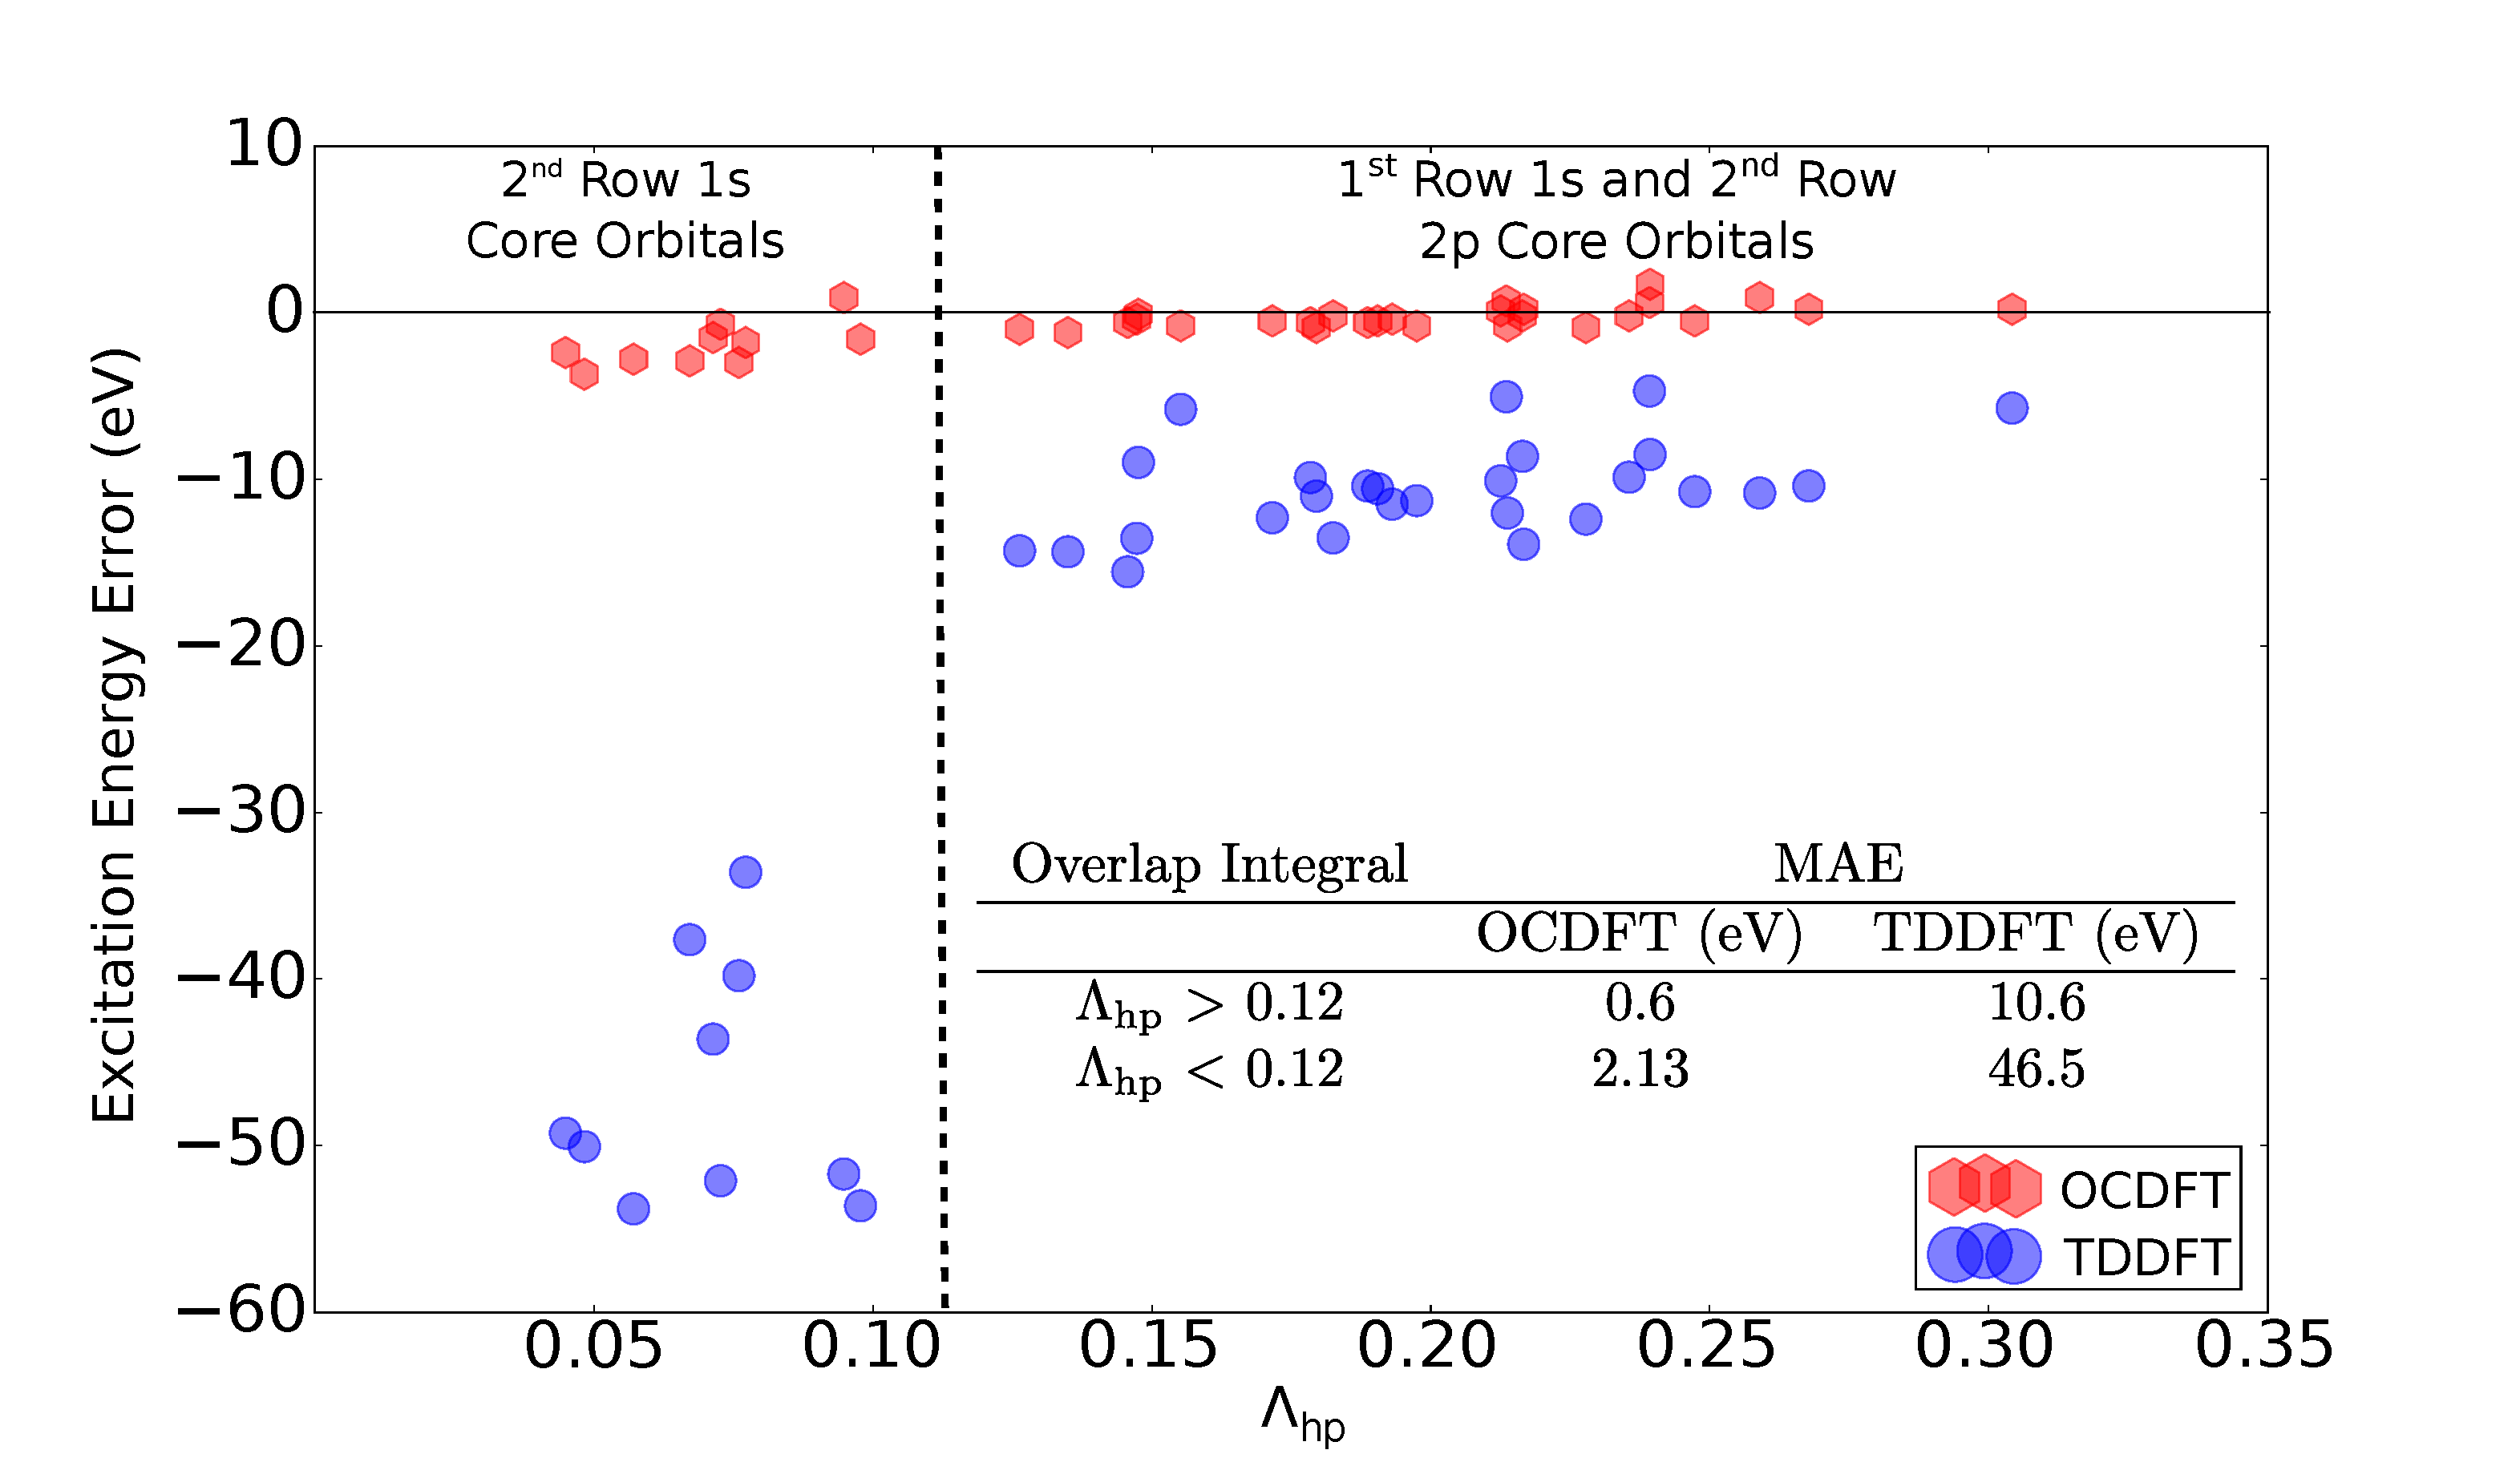
\includegraphics[scale=0.17]{scatterNEW.pdf}
\caption{Scatterplot displaying the excitation energy error as a function of orbital overlap. Excitation energies were calculated using the B3LYP functional and def2-QZVP basis set. The overlap integrals were computed with numerical grid integration making use of the Gaussian cube files produced by in Psi4 OCDFT calculations. Grids were calculated with a double zeta basis set and 0.1 grid spacing.}
\label{figure:scatter}
\end{figure}
core hole and valence particle orbitals have little overlap. The overlap between the hole and particle orbital ($\Lambda_{hp}$) is defined by the following integral:
\begin{align}
\Lambda_{hp} = &\int |\phi_h (\bf{r})||\phi_p (\bf{r})| \ d\bf{r} \\ &\text{where} \ 0 \leq \Lambda_{hp} \leq 1 , \nonumber
\end{align}
which describes the amount of overlap between the two orbitals involved. Figure \ref{figure:scatter} displays the effect that a decrease in orbital overlap has on the accuracy of the excitation energy computed with OCDFT and TDDFT. The vertical dashed line at 0.12 separates the low overlap region (containing exclusively excitations from second row 1s core orbitals) from the higher overlap region (containing exclusively excitations from first row 1s and second row 2p core orbitals). The scatterplot clearly shows that OCDFT is less sensitive to variations in the overlap. Transitioning from the low overlap region to the high overlap region the MAE increases by only 1.5 eV for OCDFT, while in the case of TDDFT the error increases drastically by 35.9 eV.\\ \\
\begin{table*}[t]
    \centering
    \begin{tabular}{lll@{\hskip 0.6in}llHH}
    \hline
    \hline
     Molecule & Excitation                     & Exp.& TDDFT & OCDFT   &     \\
     \hline
    ~         & ~                              &   &     &  & TDDFT    & OCDFT \\
    \multirow{2}{*}{SiH$_4$}        & Si 1s $\rightarrow$ $\sigma^*$     & 1842.5 & -38.4    & -1.8  & -38.9    & -2.3   \\
             & Si 2p $\rightarrow$ $\sigma^*$ & 102.8 & -4.8 & 0.6 \vspace{2mm}   & -4.1    & 1.5 \\
    \multirow{2}{*}{PH$_3$ }     & P 1s $\rightarrow$ $\sigma^*$ & 2145.8   & -44.1     & -2.9  & -44.1    & -3.2   \\
    ~         & P 2p $\rightarrow$ $\sigma^*$          & 132.3 & -5.1     & 0.7  \vspace{2mm} & -5.1    & 0.0 \\
    \multirow{4}{*}{H$_2$S}    &S 1s  $\rightarrow$ $\sigma^*$ &  2473.1 & -48.3 &  -3.0 & -48.3 & -3.8 \\
    ~         &S 1s  $\rightarrow$ 4p &  2476.3 & -52.1 &  -1.5 & -52.1 & -0.6 \\
    ~         & S 2p $\rightarrow$ $\sigma^*$ & 164.5 & -5.1    & 0.8  & -5.1    & 0.4  \\
    ~         & S 2p $\rightarrow$ 4s      & 166.5 &  -7.1    & -0.7 \vspace{2mm}   & -7.1    & -1.0 \\
    \multirow{3}{*}{SO$_2$}         &S 1s  $\rightarrow$ $\pi^*$ & 2473.8 & -50.1 & -3.7 & -51.3 & -4.5 \\
    ~         & S 1s  $\rightarrow$ 4p & 2478.4 & -49.3 & -2.4 & -50.4 & -3.2 \\
    ~         & S 2p $\rightarrow$ 4s      & 171.3 & -8.3     & -1.5 \vspace{2mm}   & -8.2    & -1.9 \\
    \multirow{3}{*}{HCl}       & Cl 1s $\rightarrow$ $\sigma^*$     & 2823.9 & -53.8     & -2.3  & -55.4    & -4.7  \\
    ~         & Cl 1s $\rightarrow$ 4p          & 2827.8 & -52.1      & -0.7   & -52.7    & -1.7  \\
    ~         & Cl 2p $\rightarrow$  $\sigma^*$    & 201.0 & -6.1 & 0.8 \vspace{2mm}  & -6.1    & 0.3 \\
    \multirow{3}{*}{Cl$_2$}      & Cl 1s $\rightarrow$ $\sigma^*$          & 2821.3   & -53.6      & -1.6   & -55.3    & -3.6   \\
    ~         & Cl 1s $\rightarrow$ 4p          & 2828.5 & -51.7    & 0.9  & -53.5     & -0.2  \\
        ~         & Cl 2p $\rightarrow$  $\sigma^*$    & 198.7 & -5.7     & -0.8 \vspace{2mm} & -5.8    & -0.3\\
    \hline
    ~         & MAE                            & ~     & 31.6      & 1.6   & 32.0     & 2.0   \\
    \end{tabular}
    \caption{Calculated core excitation energies for excitations involving 1s/2p electrons of second-row atoms. Computations were performed using the B3LYP density functional and def2-QZVP basis set, the values reported here are the deviations from the experimental value in electron volts (eV). Mean Absolute Error (MAE) is reported for each method.}
     \label{table:SecondRow}
\end{table*}
\begin{comment}
Multiple studies have concluded that the shortcoming of traditional density functionals is not the treatment of long-range interaction, but instead it is the incorrect description of the core region that leads to inaccuracy. [CITE] This problem was specifically addressed by the SRC-BLYP functional \cite{besley_time-dependent_2009} which is a flexible functional that increases the amount of Hartree-Fock exchange at short range and is identical to the long range corrected CAM-BLYP at long range. 
\end{comment}
It has been concluded that varying HF exchange parameters can vastly improve the description of core-excited states,\cite{nakata_time-dependent_2006} however here we approached the problem in a different way. With a slight augmentation to DFT derived from first principles, an accurate description of core excited states is possible without relying on varying the amount of HF exchange. 
\begin{figure}[t]
\centering
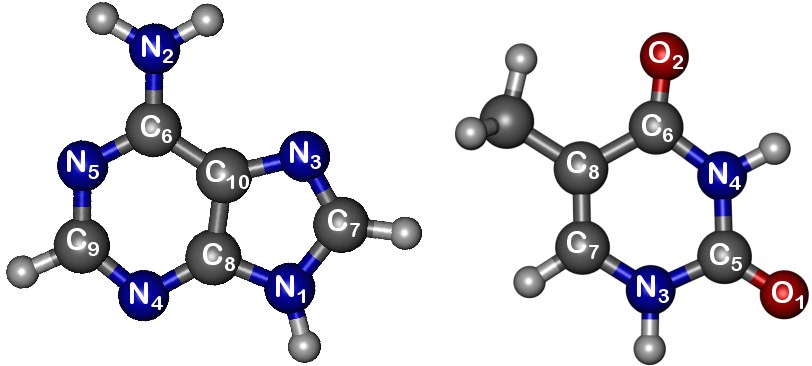
\includegraphics[scale=0.45]{adenineThymineNumbering3D.png}
\caption{Numbering scheme of adenine (left) and thymine(right), atoms are assigned a number based on decreasing Hartree-Fock orbital energy of their 1s core orbital. }
\end{figure}
\begin{figure}[!ht]
\centering
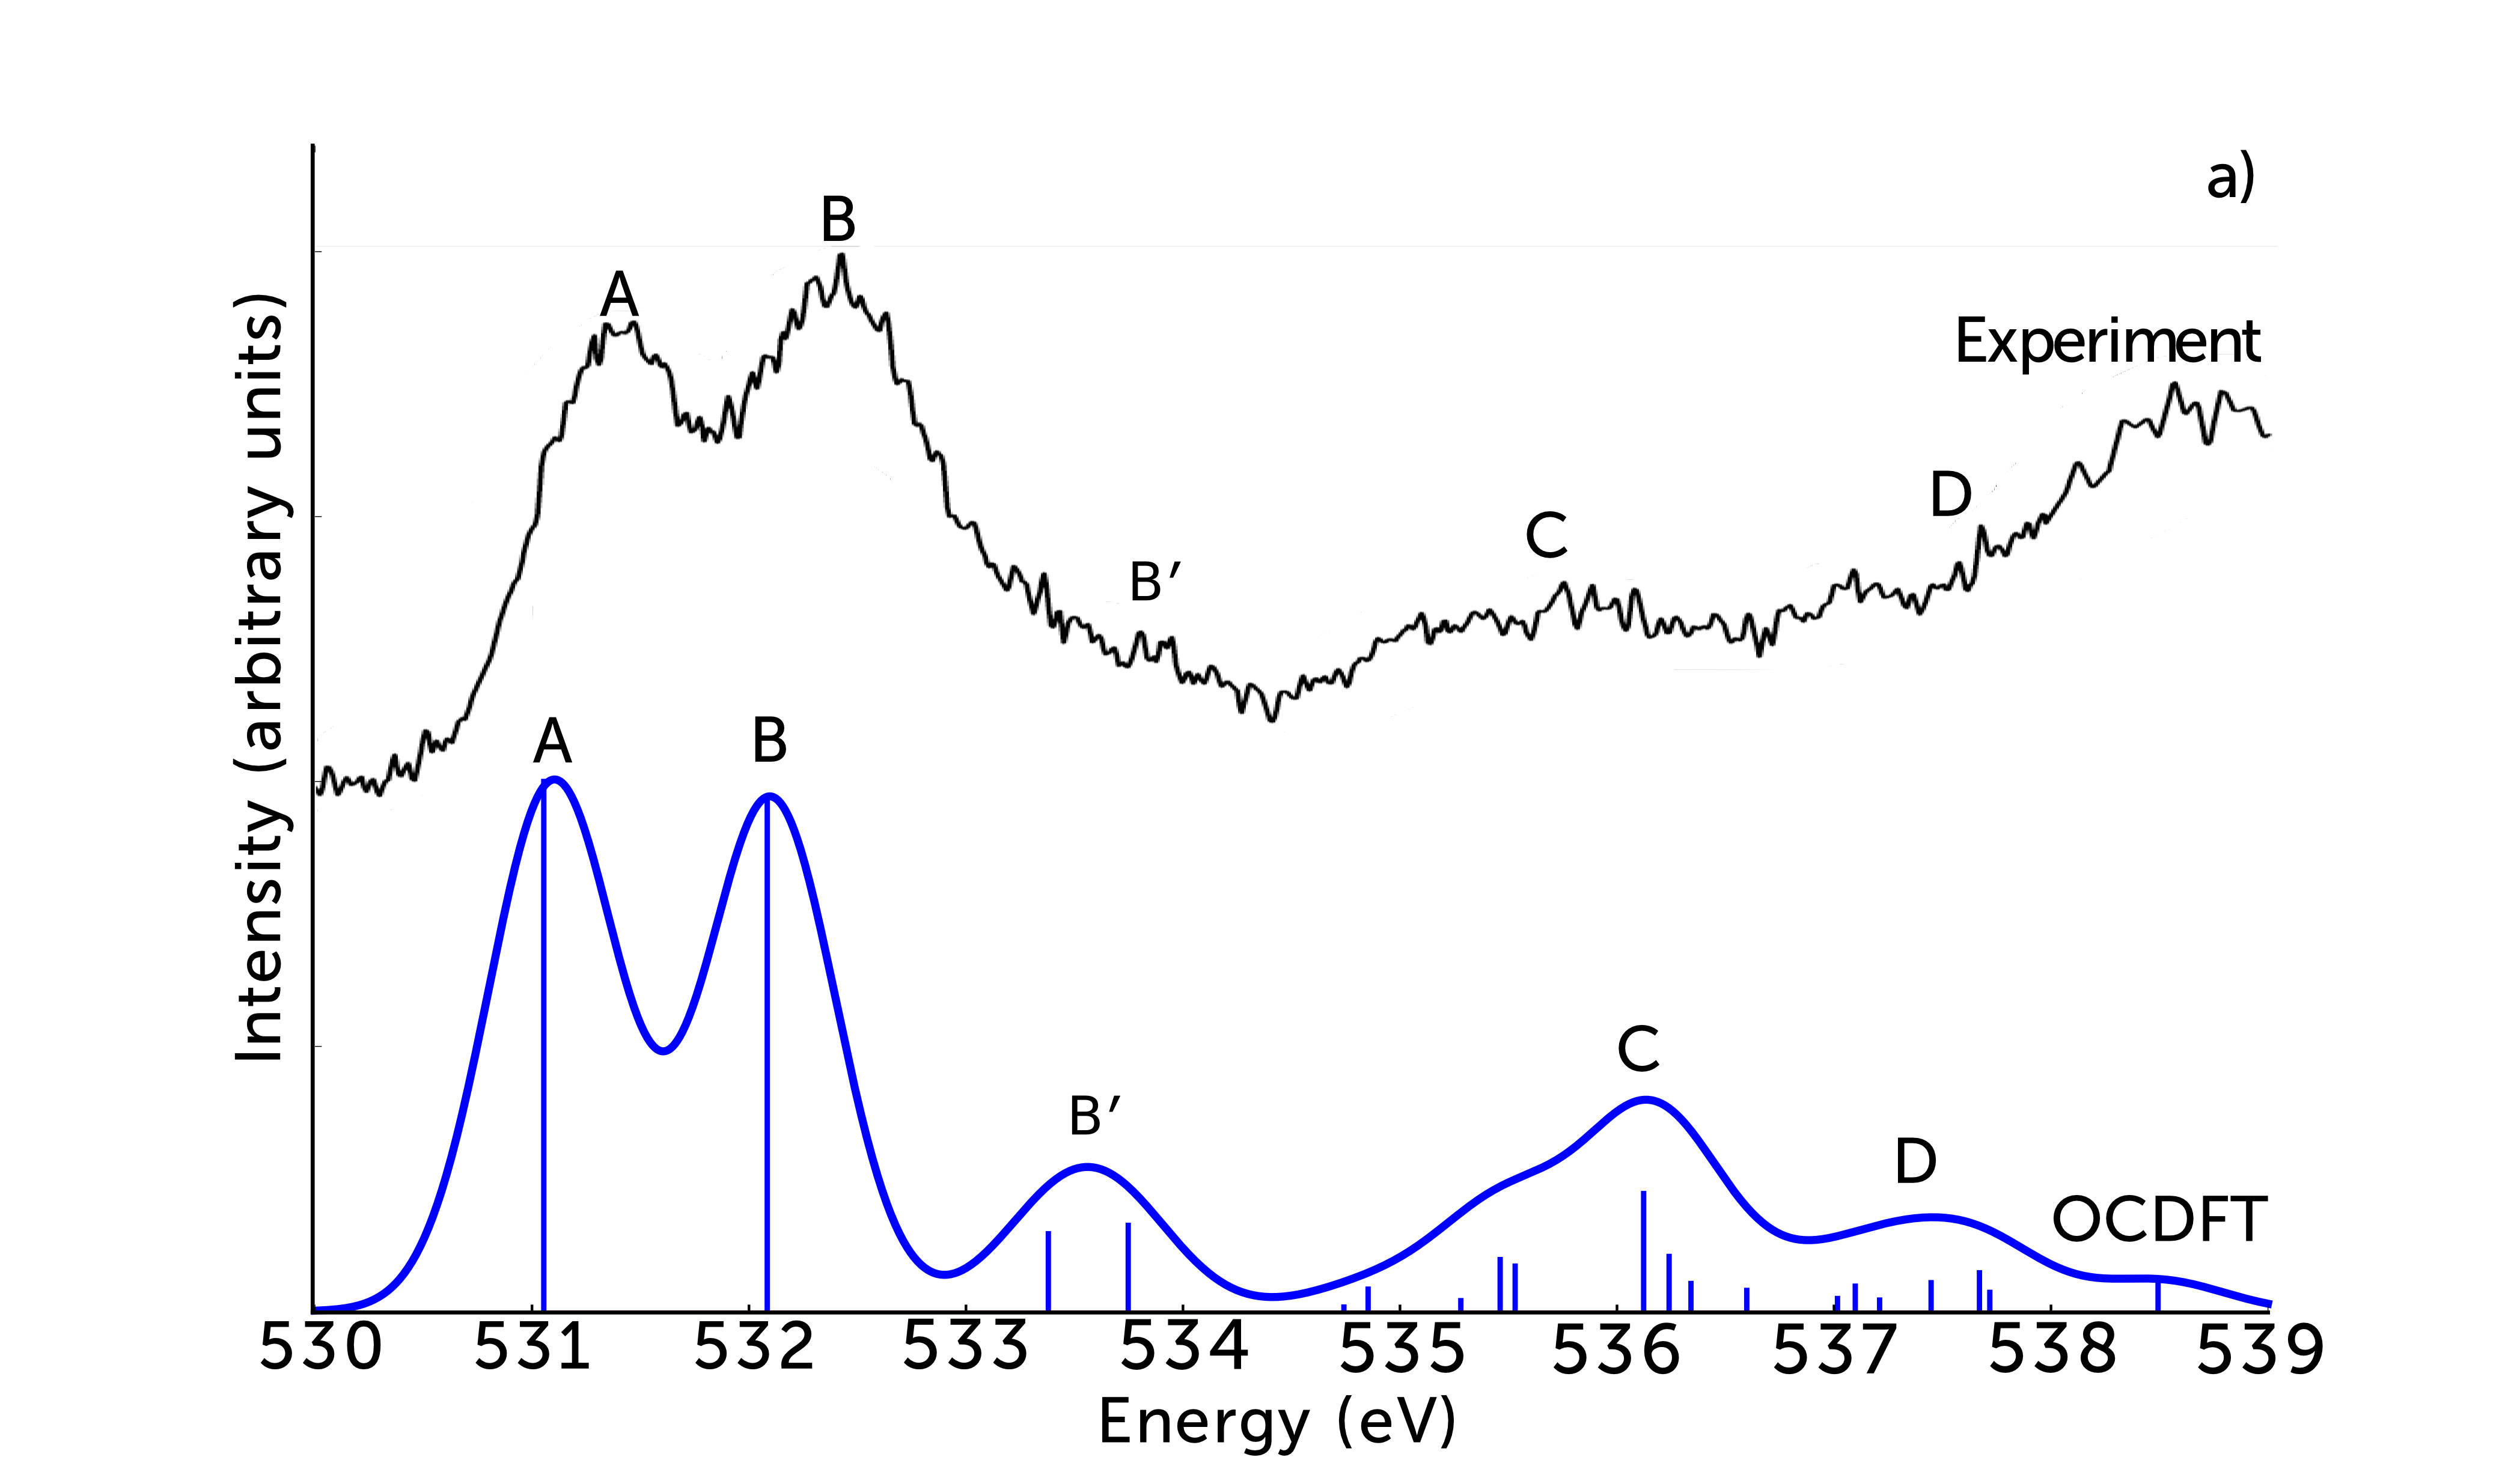
\includegraphics[scale=0.15]{ThymineOKexperiment.png}\\
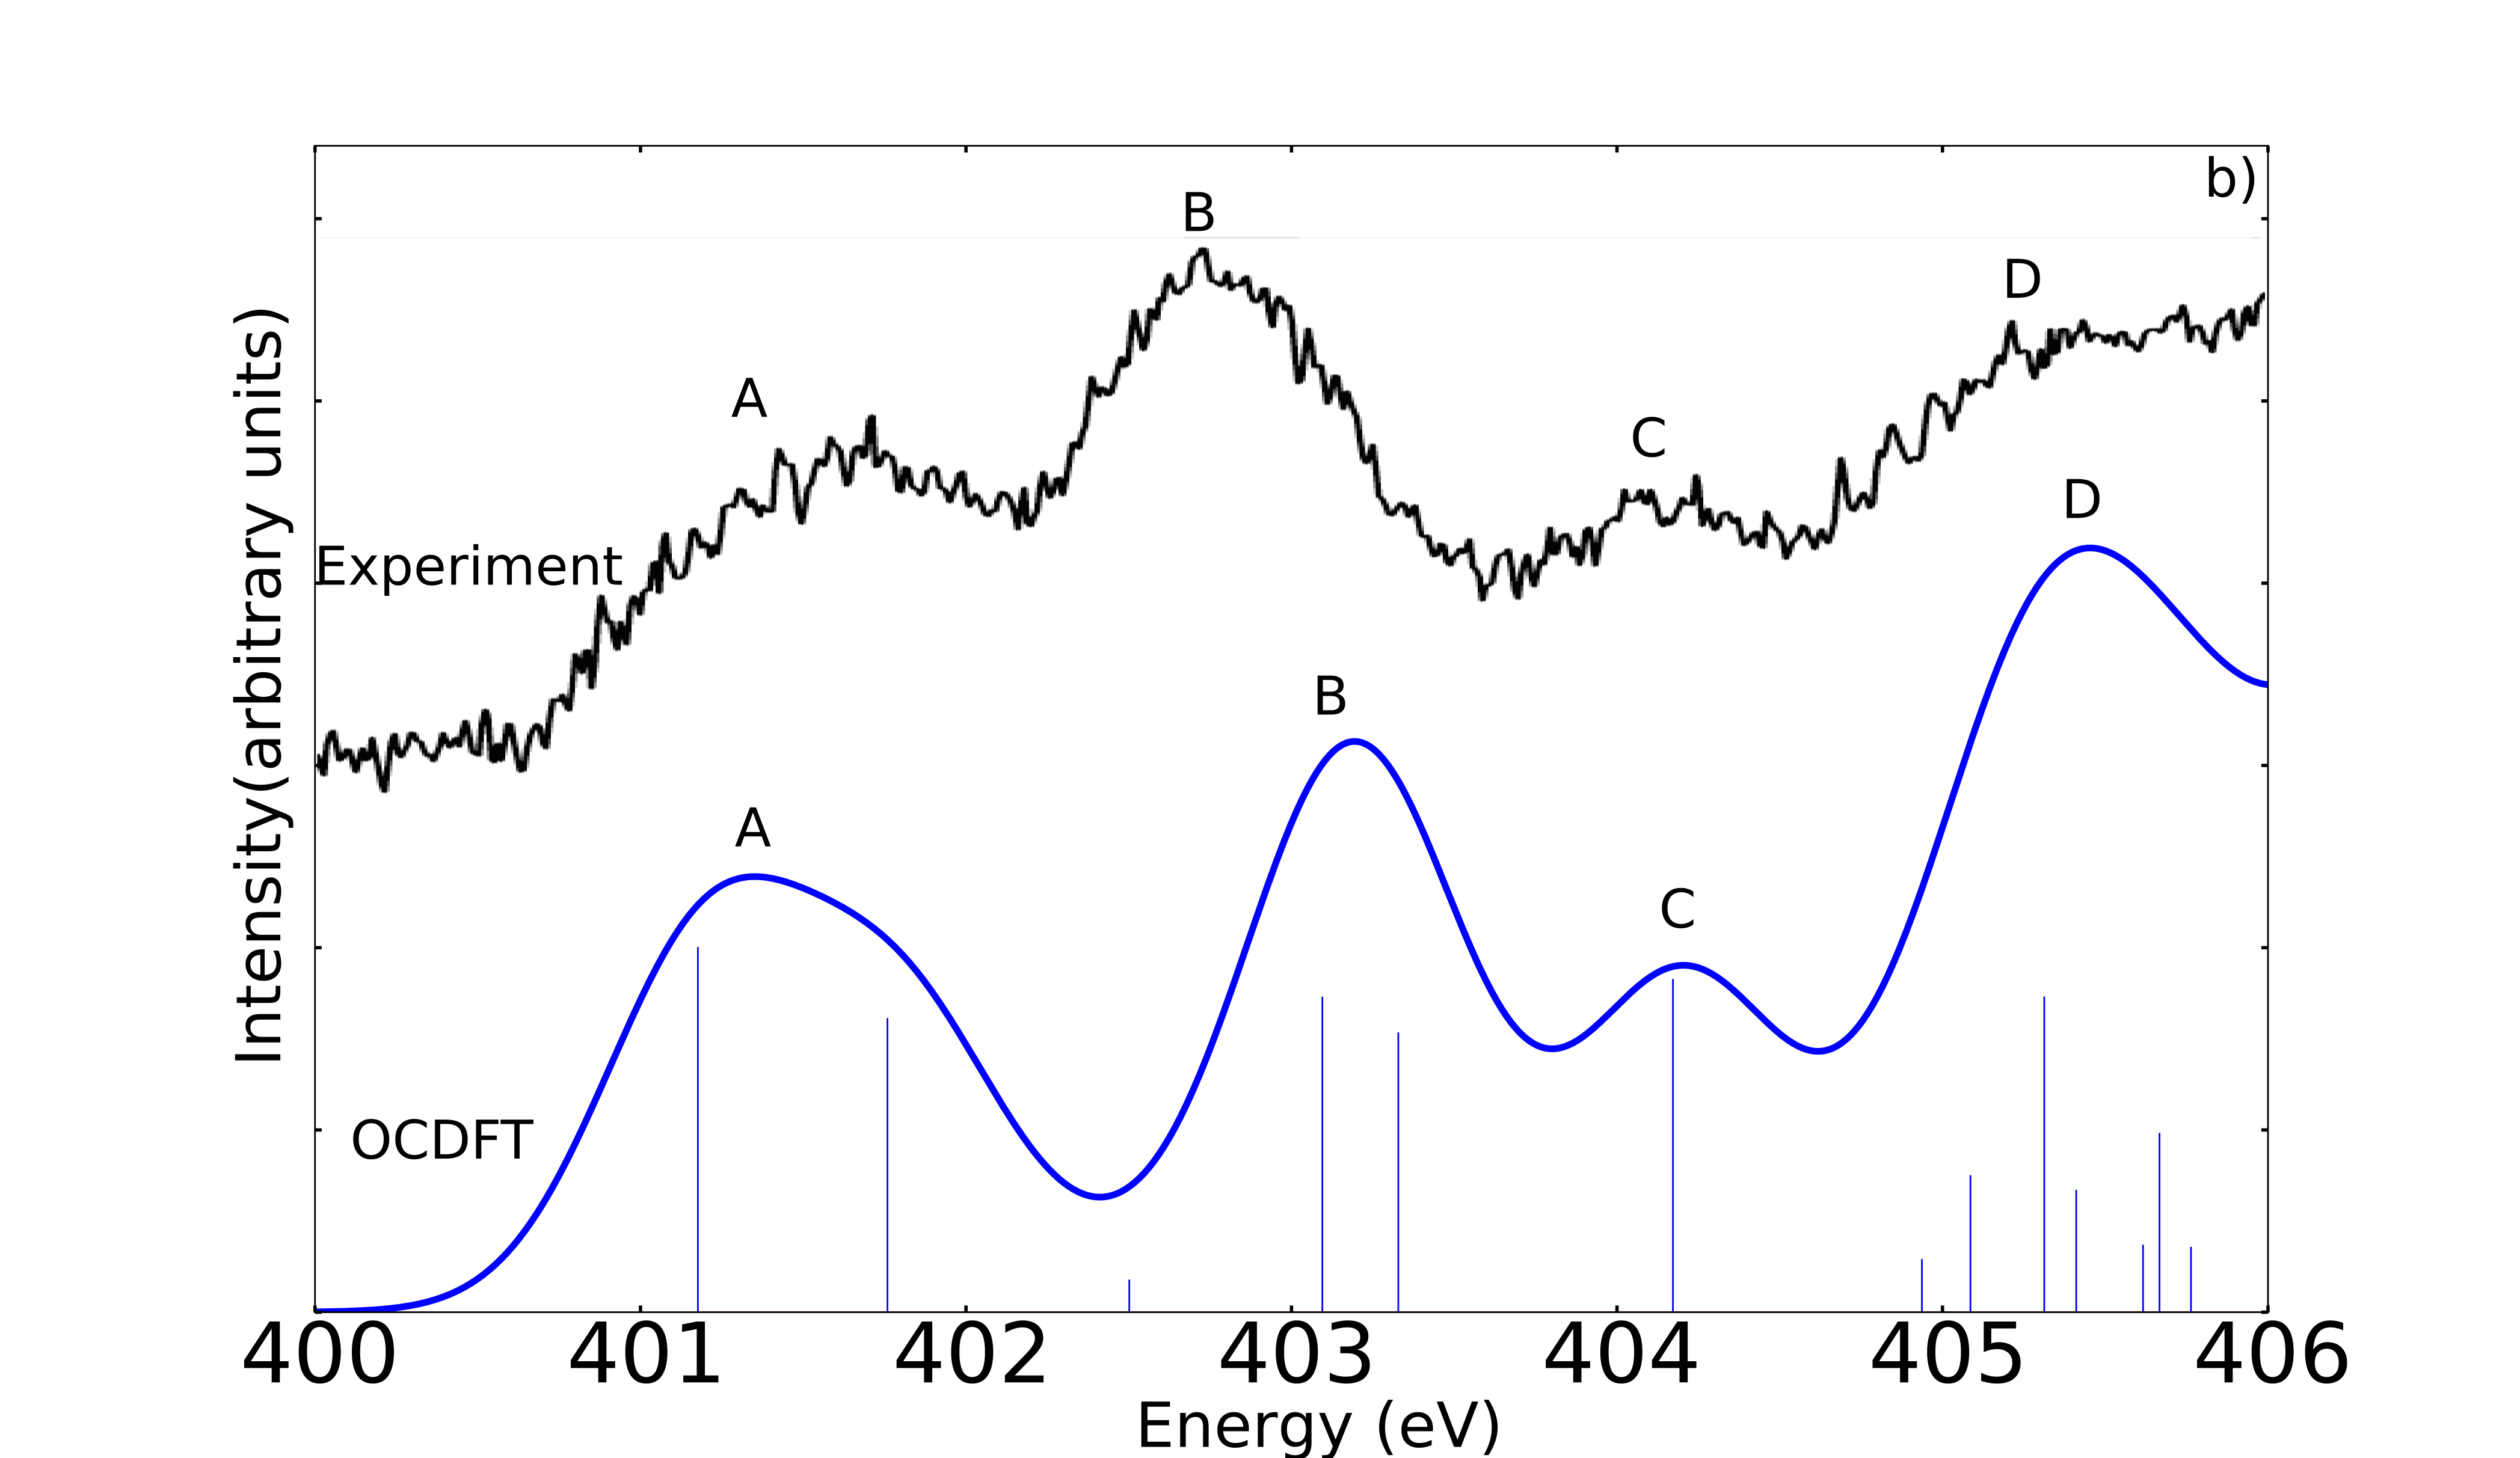
\includegraphics[scale=0.15]{ThymineNKexperiment.png} \\
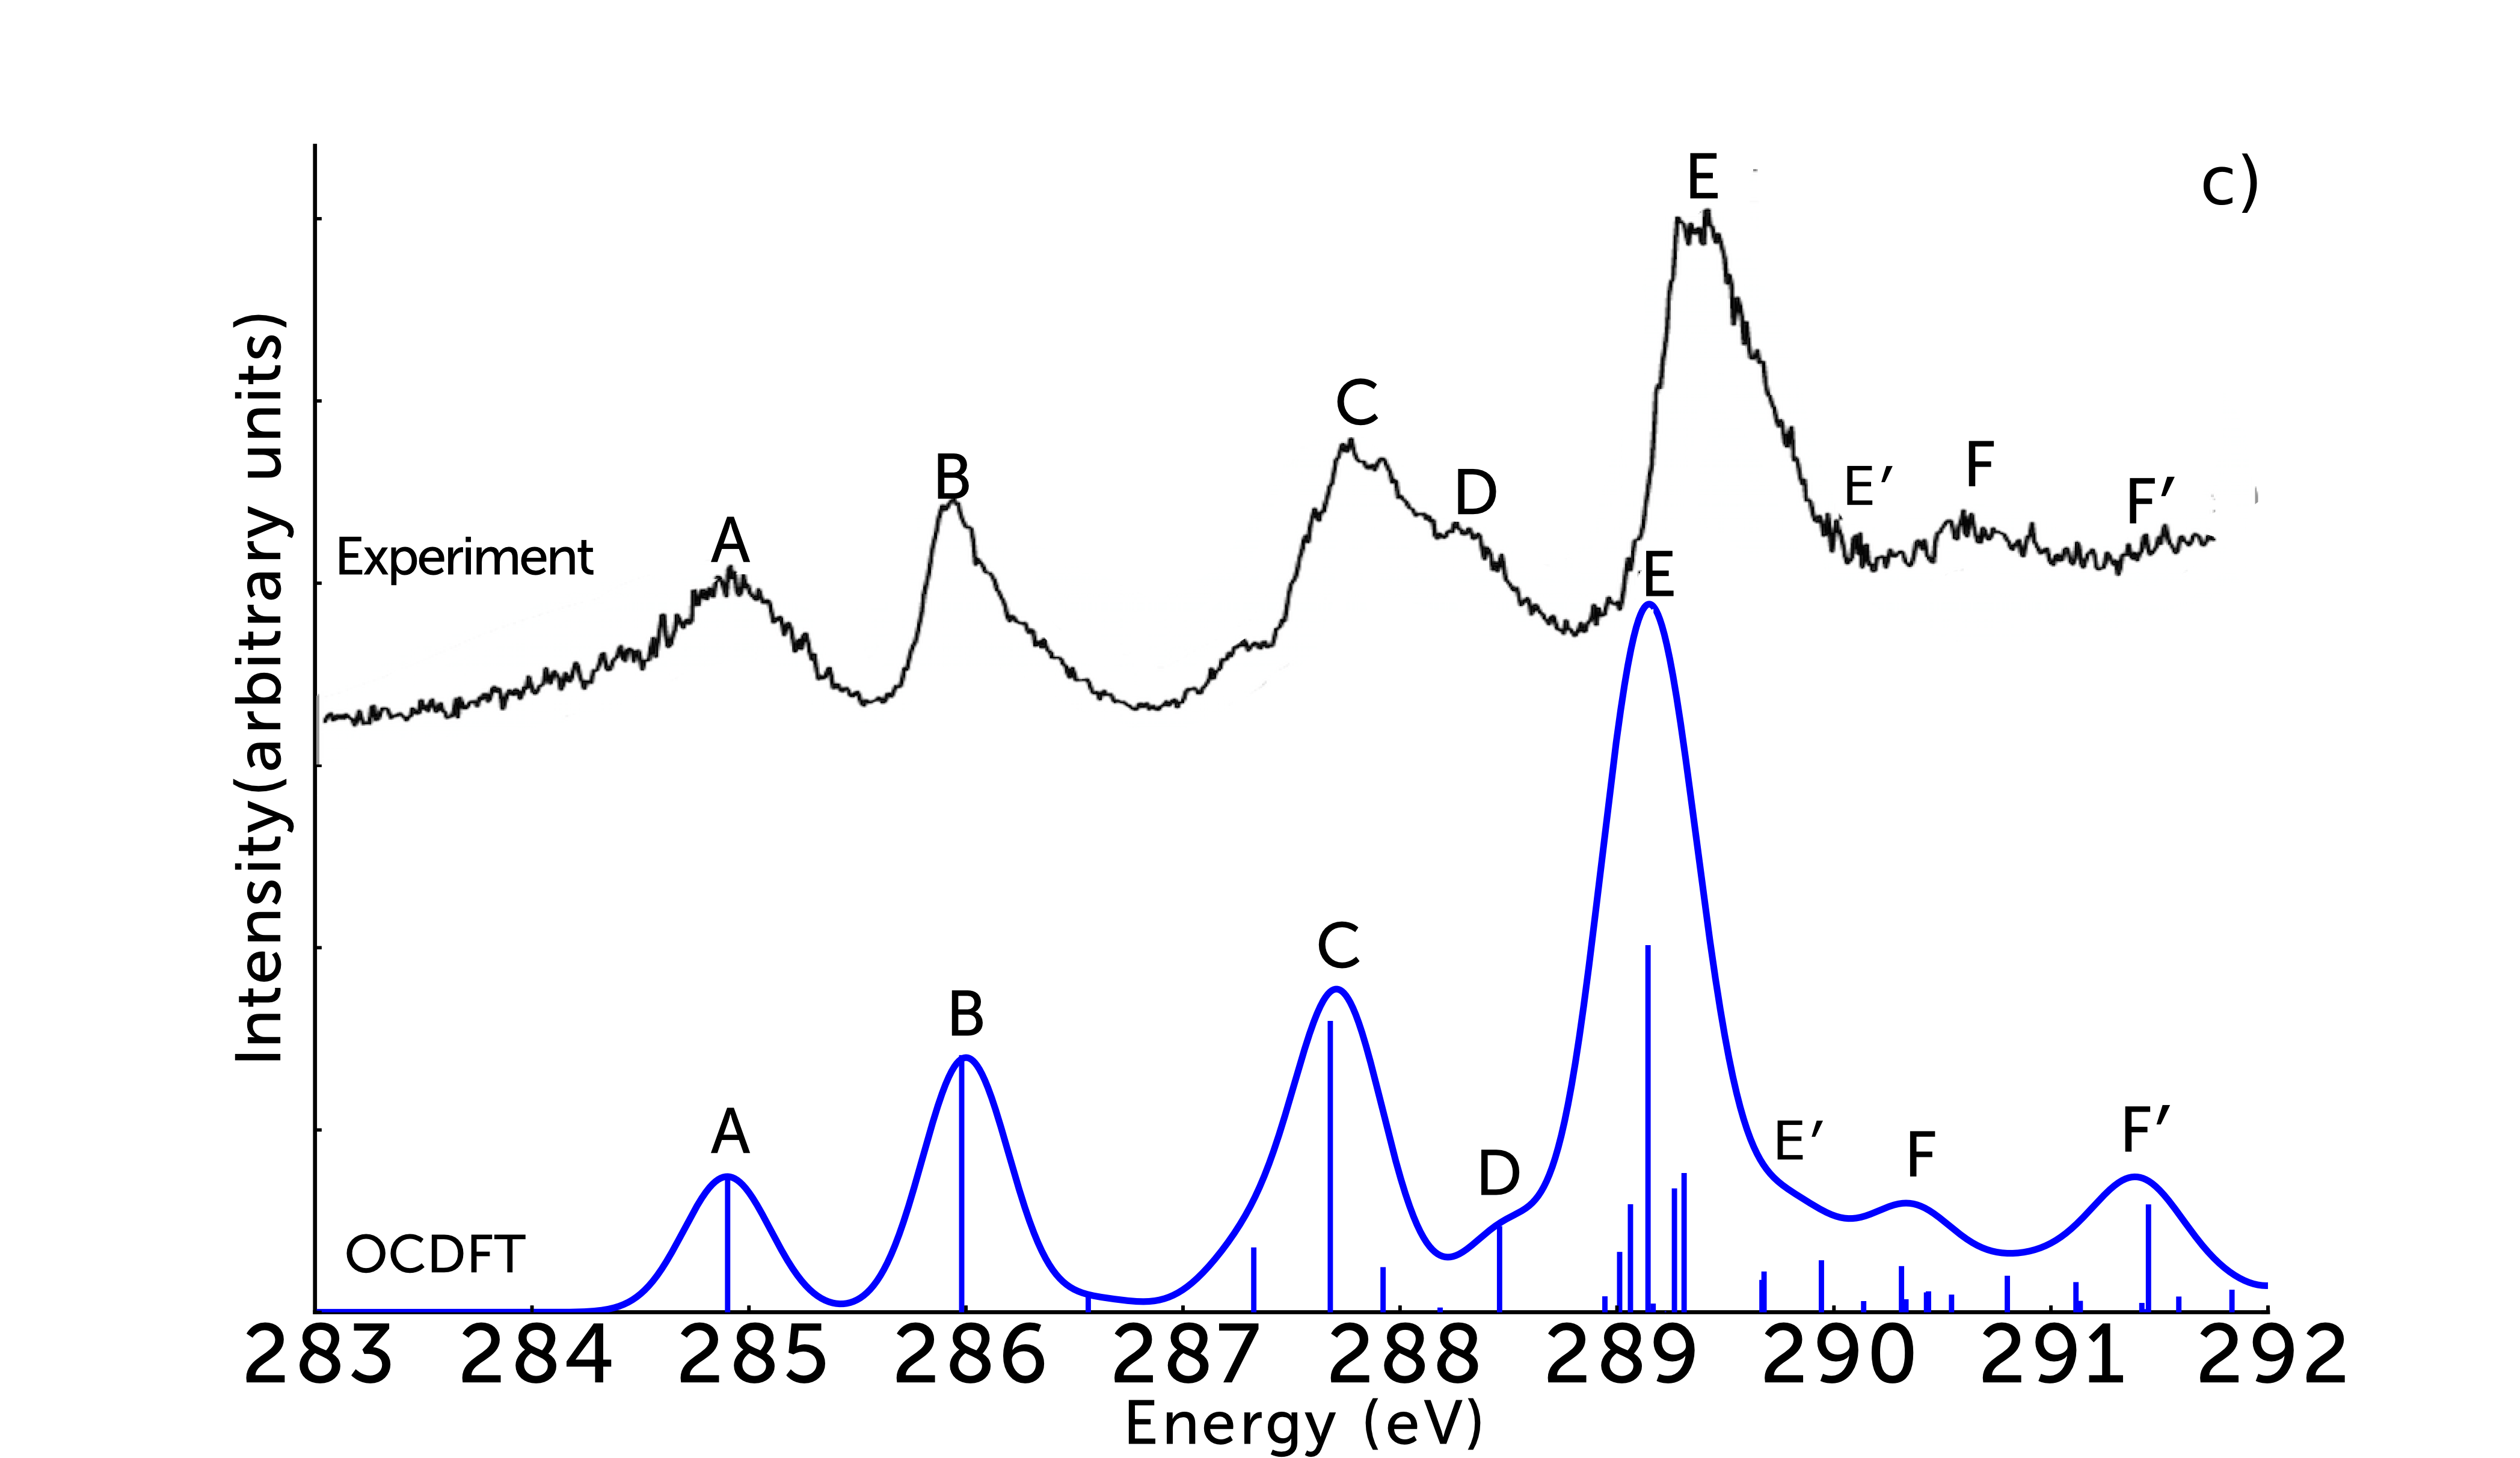
\includegraphics[scale=0.15]{ThymineCKexperiment.png}
\caption{Core excited states for thymine computed using B3LYP functional and def2-TZVP basis set. Spectra is composed of convoluted Gaussians with a Full Width at Half Maximum (FWHM) of 0.3 eVs of the (a) oxygen K-edge, (b) nitrogen K-edge, and (c) carbon K-edge. Experimental spectra is from reference [CITE].}
\label{figure:Thymine}
\end{figure}
\subsection{Application to Nucleobases: Thymine and Adenine Near-Edge Spectra}

\begin{table}
\centering
    \begin{tabular}{c@{\hskip 0.22in}c@{\hskip 0.22in}c@{\hskip 0.52in}c@{\hskip 0.22in}c@{\hskip 0.22in}c}
    \hline
    \hline
  \multicolumn{3}{c}{OCDFT} &\multicolumn{2}{c}{Experiment} \\
  \hline
  Assignment & $\omega_{fi}$ & f$_{rel}$ & Peak &  $\omega_{fi}$   \\
  \hline
   O$_2$ $\rightarrow$ $\pi_2^*$ & 531.05 & 1.000 &  A & 531.4
   \vspace{2mm}\\
   O$_1$ $\rightarrow$ $\pi_1^*$ & 532.08 & 0.968 &  B & 532.3 
   \vspace{2mm}\\
   O$_1$ $\rightarrow$ $\pi_2^*$ & 533.38 & 0.146 & \multirow{2}{*}{ B$^{\prime}$} \\
   O$_2$ $\rightarrow$ $\pi_1^*$ & 533.75 & 0.162 &  \multirow{9}{*}{C} & \multirow{9}{*}{535.7}
   \vspace{2mm}\\
   O$_1$ $\rightarrow$ 3s & 534.74 & 0.008 \\
   O$_2$ $\rightarrow$ 3s & 534.85 & 0.042 \\
   O$_2$ $\rightarrow$ 3p & 535.28 & 0.020\\
   O$_1$ $\rightarrow$ 3p & 535.46 & 0.098\\
   O$_2$ $\rightarrow$ 3p & 535.53 & 0.085\\
   O$_1$ $\rightarrow$ 3p & 536.12 & 0.222\\
   O$_2$ $\rightarrow$ 4p & 536.24 & 0.103\\
   O$_2$ $\rightarrow$ $\pi_3^*$ & 536.34 & \ 0.052
   \vspace{2mm}\\
   O$_1$ $\rightarrow$ 4s & 536.60 & 0.039 & \multirow{6}{*}{D} & \multirow{6}{*}{537.1}\\
   O$_2$ $\rightarrow$ 4p & 537.02 & 0.024\\
   O$_1$ $\rightarrow$ $\pi_3^*$ & 537.10 & 0.047\\
   O$_1$ $\rightarrow$ 4p & 537.45 & 0.054\\
   O$_2$ $\rightarrow$ 4p & 537.67 & 0.073\\
   O$_2$ $\rightarrow$ 4p & 537.72 & 0.035
   \vspace{2mm}\\
   O$_1$ $\rightarrow$ 5p & 538.49 & 0.058 & \ D$^{\prime}$\\
   \hline
  \end{tabular}
      \caption{Calculated and experimental thymine core excitation energies in eV are shown in the table. All excitations originate from the 1s orbital on the specified atom. \\
  $^{\ddagger}$Experimental value for this transition is inconclusive, value shown here was calculated using ADC(2)}
  \label{figure:MOs}
  \end{table}
  The nucleobases are vastly important organic molecules that play a key biological role as the building blocks of DNA and recently show promise as potential materials for electronic/technological applications [CITE]. Early theoretical studies characterized the electronic structure of the base pairs using low-level methodologies, such as Huckel theory [CITE] and linear combination of atomic orbitals (LCAO)-SCF methods [CITE]. Early X-ray experiments on nucleobases were largely scattering and diffraction based techniques[CITE], it wasn't until 1992 that the first near-edge absorption experiments were performed by Sudipa Mitra Kirtley et al.[CITE] In this study they selectively characterized the nitrogen environment and revealed the useful sensitivity of the 1s $\rightarrow$ $\pi^*$ resonances to their surrounding chemical environment. Modern experiments have moved beyond simple characterization and aim to probe interactions with surfaces and other applications.  A wide array of computational methods have been used to compute the near-edge structure of these molecules, including: restricted active space SCF (RASSCF)[CITE], improved virtual orbital SCF (IVO-SCF)[CITE], a complex polarization propagator method (CPP) [CITE], SIC-DFT[CITE], $\Delta$MP2[CITE], equivalent core approximation (ECA) method[CITE], and algebraic diagrammatic construction [ADC(2)][CITE]. Due to TDDFT's consistent underestimation of core excitation energies, it is a very limited tool for studying these types of molecules. Although it can be useful in predicting energy gaps or other relative trends[CITE], It must rely on experimental results in order to obtain any quantitatively useful excitation energies.
  \begin{comment}
  \begin{table}[ht]
    \renewcommand{\arraystretch}{0.01}
    \scalebox{1}{
    \begin{tabular}{cccc@{\hskip 0.6in}c}
    \hline
    \hline
     Atom & Exp. &  OCDFT    & $\phi_h$ & $\phi_p$     \\
     \hline
     \\
    C$_6$  & 287.4 & 287.3 & \includegraphics[scale=0.035]{Ade_C6.pdf} & \includegraphics[scale=0.035]{Ade_Pi_star6.pdf}
    \\
    C$_7$  & 286.8 & 286.9 & \includegraphics[scale=0.035]{Ade_C7.pdf} & \includegraphics[scale=0.035]{Ade_Pi_star7.pdf}
    \\
    C$_8$  & 287.4 & 287.4 & \includegraphics[scale=0.035]{Ade_C8.pdf} & \includegraphics[scale=0.035]{Ade_Pi_star8.pdf}
        \\
    C$_9$  & 286.4 & 286.5 & \includegraphics[scale=0.035]{Ade_C9.pdf} & \includegraphics[scale=0.035]{Ade_Pi_star9.pdf}
        \\
    C$_10$  & 286.0 & 286.3 & \includegraphics[scale=0.035]{Ade_C10.pdf} & \includegraphics[scale=0.035]{Ade_Pi_star10.pdf}
          \end{tabular}
}
\caption{Carbon 1s $\rightarrow$ $\pi^*$ excitations in adenine. All calculations were performed at the B3LYP level of theory using the def2-TZVP basis set. All excitation energies shown are in electron volts (eV)}
\end{table}
\end{comment}
\subsubsection{Thymine}
  \begin{figure}[ht!]
  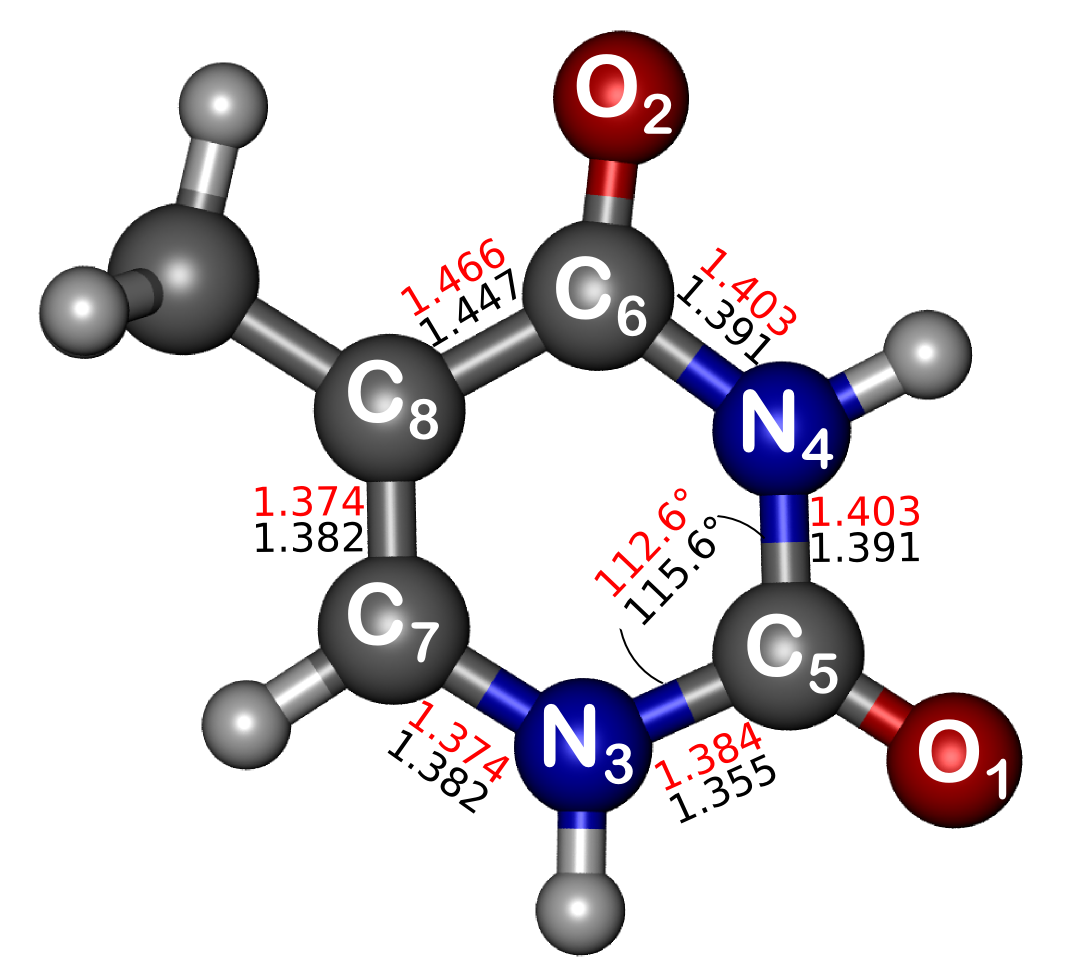
\includegraphics[scale=0.60]{g130.png} 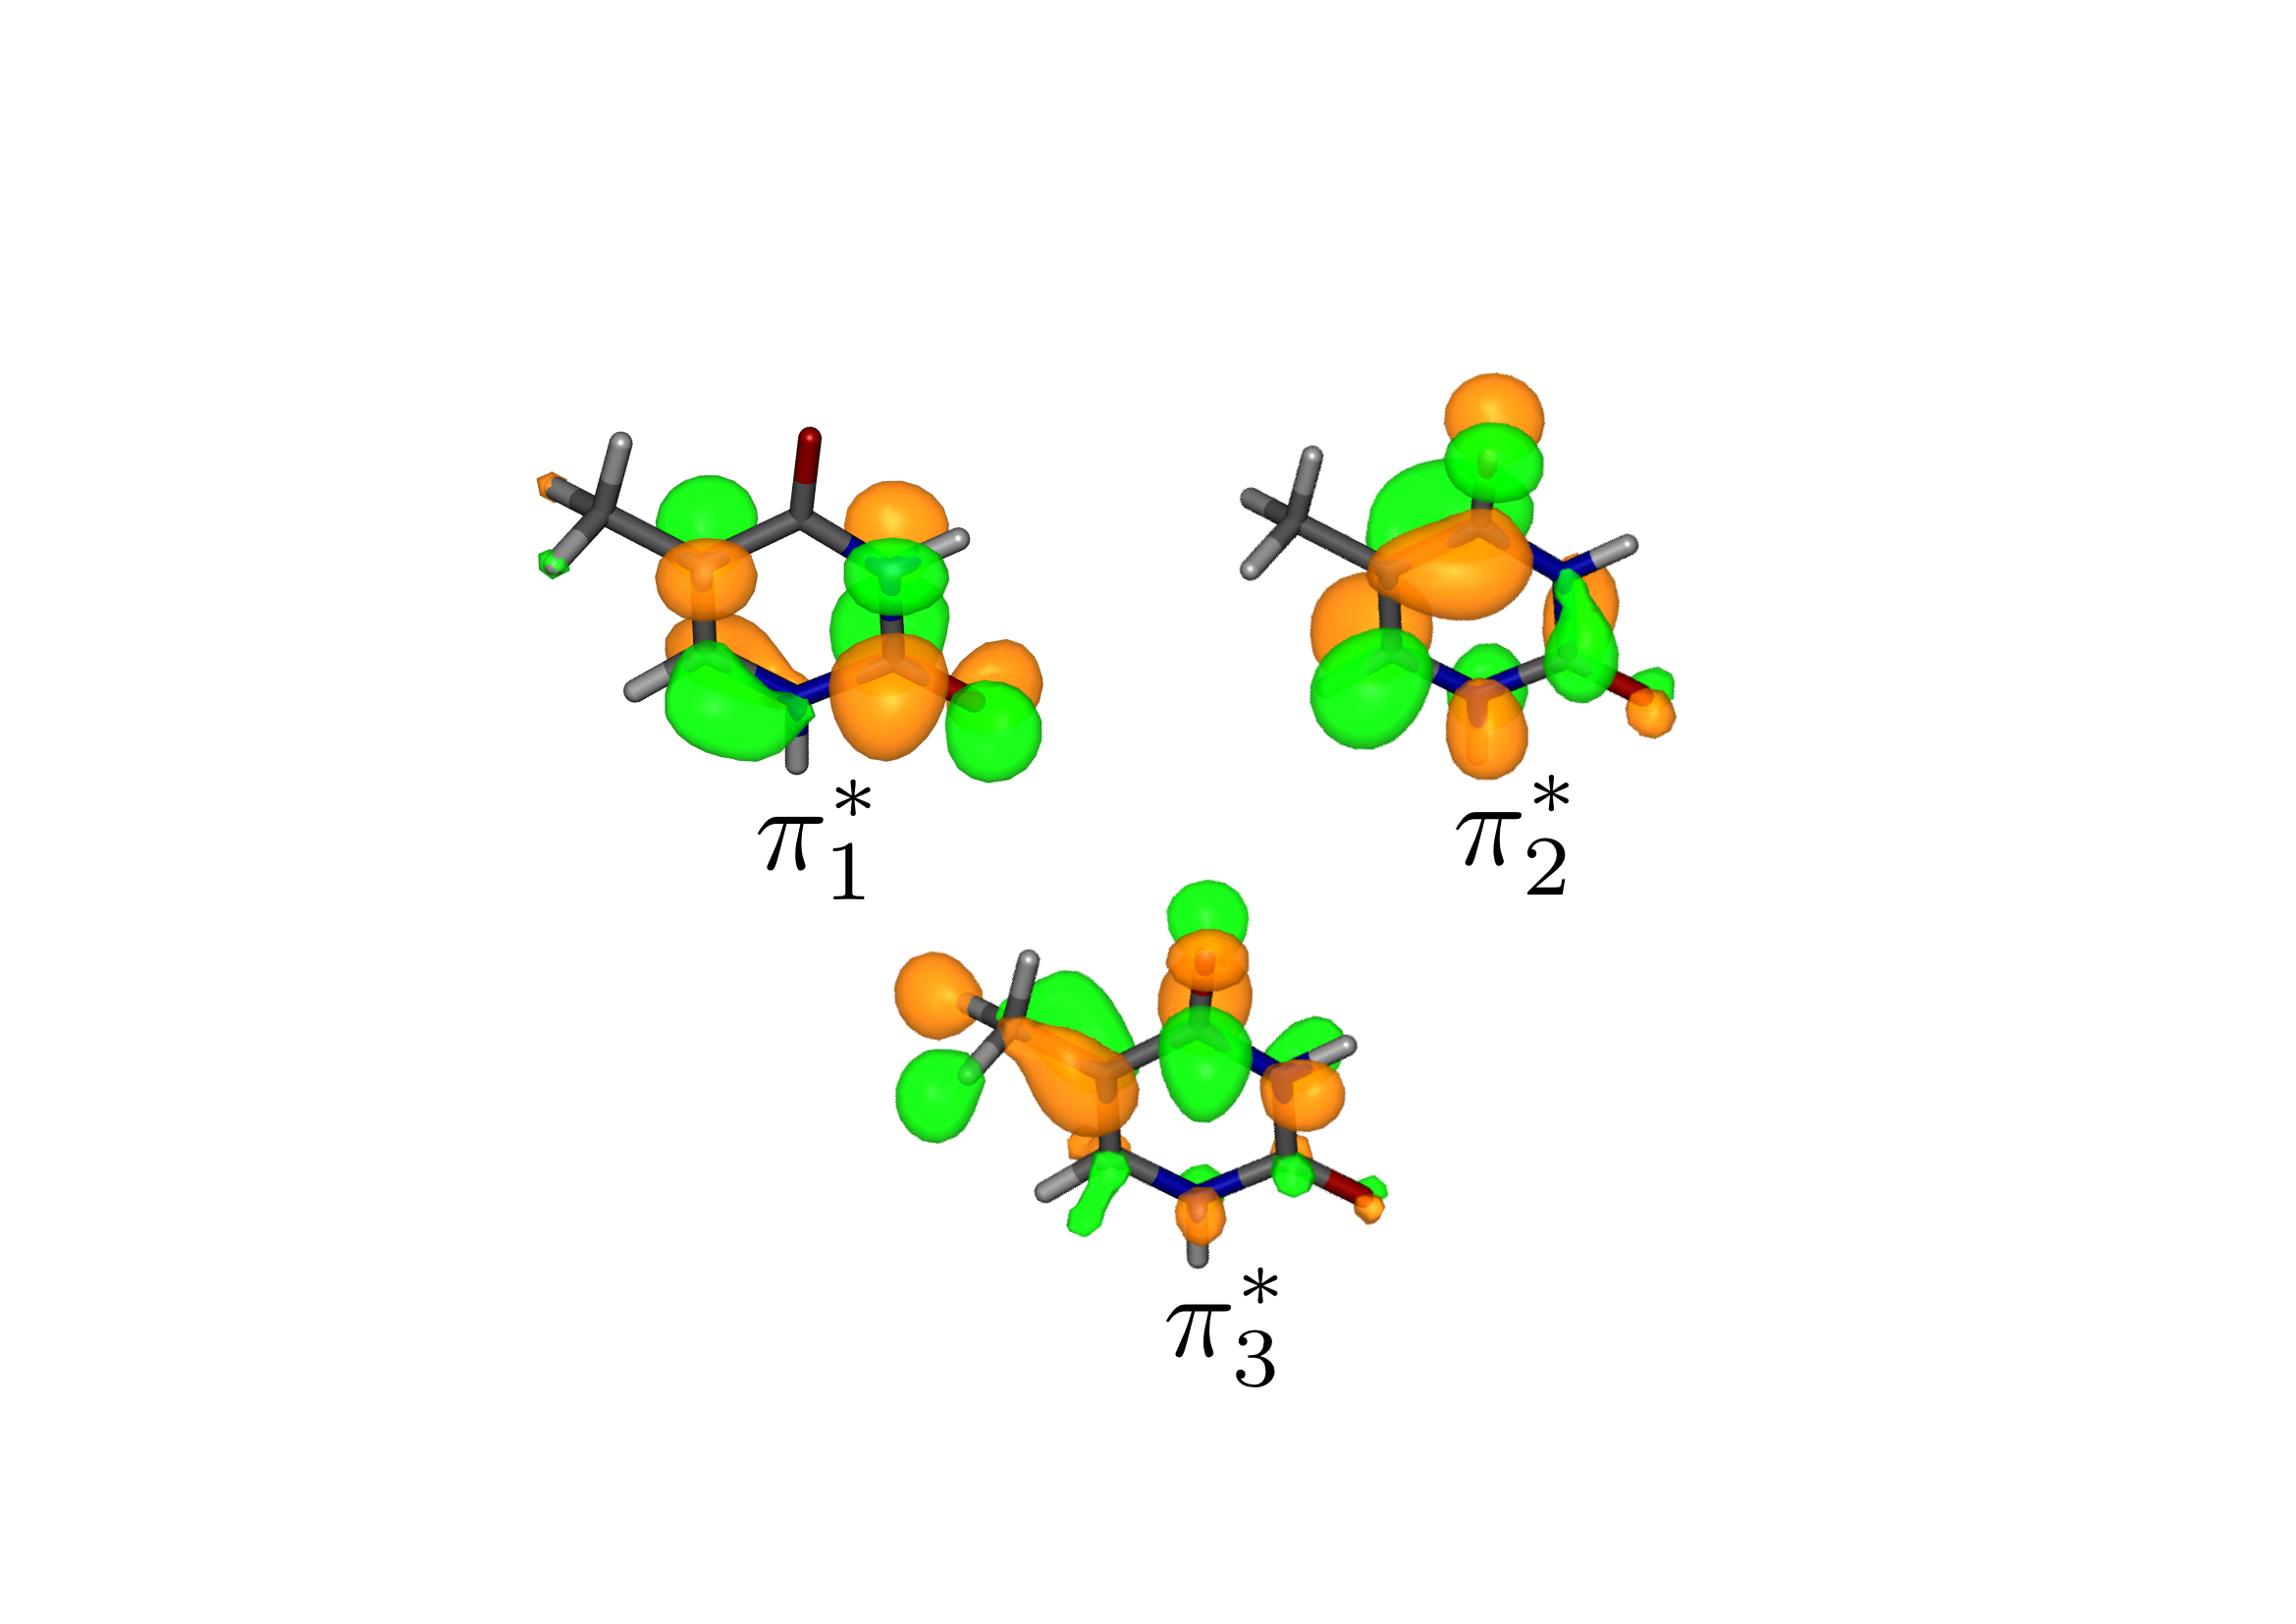
\includegraphics[scale=0.4]{particleorbitals.png}
  \caption{(Left) Optimized geometry and numbering scheme for thymine. Atoms are numbered based on the Hartree-Fock energy of their respective 1s orbitals starting with the highest energy core (O$_1$). The top number (in red) is the calculated bond length/angle computed at the B3LYP level of theory, while the bottom number (in black) shows values from the experimental crystal structure.[CITE] (Right) Relevant $\pi^*$ particle orbitals for thymine}
  \end{figure}
  \ In this section the O, N, and C core excitation spectra of thymine will be predicted using OCDFT in tandem with B3LYP.  A basis set of triple zeta quality (def2-TZVP) was employed in the calculation of all core-excitations. Peak intensities were approximated by taking the transition dipole moments ($\mu_i$) and calculating an oscillator strength ($f_{osc} $) for each transition ($\omega_{i}$)
  \begin{align}
  f_{osc} = \frac{2}{3} (\mu_x^2 + \mu_y^2 + \mu_z^2) \omega_{i}
  \end{align}
Equation 15 yields the absolute oscillator strength ($f_{abs}$) for a given transition. The intensity of the spectra is then scaled relative to the most intense peak, we will refer to these scaled values as the ``relative oscillator strength'' ($f_{rel}$). The peaks are represented by convoluted gaussians centered around the frequency of each calculated transition, each gaussian has a FWHM between 0.1 - 0.4 eV in order to simulate natural spectroscopic broadening effects.  The geometry was optimized at the B3LYP level of theory and shows reasonable agreement with the experimental crystal structure reported by Raymond Gerdil. [CITE] The largest deviation from the experimental structure , with regard to bond length is 0.03 $\AA$, while the bond angles agree within 3$^{\circ}$. Table \ref{figure:MOs} displays all O, N, and C core-excitation energies, their absolute oscillator strength, and the experimental peak assignments/excitation energies. The authors would like to emphasize that the computed OCDFT spectra shown have not been shifted from their original value, the calculated energies displayed in this section are direct solutions of our OCDFT implementation. \\
Figure \ref{figure:Thymine}a displays the experimental and theoretical spectra of thymine at the oxygen K-edge. The low energy regime of the oxygen K-edge is dominated by two high intensity peaks, both resulting from distinct core-valence excitations. Peak A results from the transition O$_2$ $\rightarrow$ $\pi^*_2$, while Peak B results from the transition O$_1$ $\rightarrow$ $\pi^*_1$ with a peak intensity that is roughly equal to that of Peak A. Experimentally, Peaks A and B are centered at 531.4 eV and 532.3 eV respectively, these excitation energies are predicted well by OCDFT to within 0.3 eV of the experimental peak assignments. The  O$_2$ $\rightarrow$ $\pi_2^*$ transition is predicted as the peak of highest intensity with an f$_{abs}$ of 0.016031, these results are consistent with the ADC(2) analysis performed by Plekan et al. The shoulder feature B$^{\prime}$ is composed of O$_1$ $\rightarrow$ $\pi^*_2$ and O$_2$ $\rightarrow$ $\pi^*_1$ and is predicted by OCDFT to have a fairly strong oscillator strength. This shoulder feature is completely absent from the ADC(2) spectra. However, a more recent study by Wenzel, Wormit, and Dreuw [CITE] uses a core-valence separation (CVS) approximation to the ADC(2) working equations [CVS-ADC(2)] and predicts three excitations in this shoulder region B$^{\prime}$, all with f$_{abs}$ $<$ 0.001. These weaker oscillator strengths predicted by CVS-ADC(2) are more consistent with the experimental peak profile. Excitations of weaker intensity are characteristic of the higher energy regime of the K-Edge and presents itself in many other situations [CITE], multiple experiments have attributed the weak intensities in this region to mixing of core-valence excited states with Rydberg excited states of similar energy.[CITE] This strong mixing causes the character of each individual excitation to be spread out over several different final states, resulting in highly disordered peaks of weak intensity. The dissonance in this region of the spectra makes it difficult to classify specific transitions experimentally. OCDFT results show that Peak C is largely composed of a mixture of 3s, 3p, and 4p Rydberg excitations within an energy interval of 534.7 to 536.4 eV. While the majority of the contributions to Peak D, are 4s and 4p excitations all with f$_{\text{rel}}$ $<$ 0.1. Peaks C and D both contain $\pi^*_3$ character, however the contributions from these resonances are weak and overshadowed by multiple Rydberg transitions in both cases. A small shoulder D$^{\prime}$ resulting from an excitation of O$_1$ $\rightarrow$ 5p is predicted by our method and is consistent with the tailing motif at the end of the spectra. \\
\begin{table}
\centering
    \begin{tabular}{c@{\hskip 0.22in}c@{\hskip 0.22in}c@{\hskip 0.52in}c@{\hskip 0.22in}c@{\hskip 0.22in}c}
    \hline
    \hline
  \multicolumn{3}{c}{OCDFT} &\multicolumn{2}{c}{Experiment} \\
  \hline
  Assignment & $\omega_{fi}$ & f$_{rel}$ & Peak &  $\omega_{fi}$   \\
  \hline
   N$_4$ $\rightarrow$ $\pi_2^*$ & 401.18 & 1.000 &  \multirow{2}{*}{A} &\multirow{2}{*}{401.7}\\
   N$_3$ $\rightarrow$ $\pi_2^*$ & 401.76 & \ 0.805
   \vspace{2mm}\\
   N$_4$ $\rightarrow$ $\pi_1^*$ & 402.50 & 0.087 & \multirow{3}{*}{B} & \multirow{3}{*}{402.7}\\
   N$_3$ $\rightarrow$ 3s & 403.09 & 0.863\\
   N$_4$ $\rightarrow$ 3s & 403.33 & \ 0.765 
   \vspace{2mm}\\
   N$_4$ $\rightarrow$ 3p & 404.17 & 0.912 & C & 404.1 
   \vspace{2mm}\\
   N$_4$ $\rightarrow$ 4p & 404.94 & 0.144 & \multirow{6}{*}{D} & \multirow{6}{*}{405.5}\\
   N$_3$ $\rightarrow$ 3p & 405.09 & 0.373\\
   N$_4$ $\rightarrow$ $\pi_3^*$ & 405.31 & 0.864\\
   N$_3$ $\rightarrow$ 3s & 405.41 & 0.333\\
   N$_4$ $\rightarrow$ 4p & 405.61 & 0.183\\
   N$_3$ $\rightarrow$ $\pi_1^*$& 405.66 & 0.490\\
   N$_3$ $\rightarrow$ 4p & 405.76 & 0.177\\
   \hline
  \end{tabular}
      \caption{Calculated and experimental thymine core excitation energies in eV are shown in the table. All excitations originate from the 1s orbital on the specified atom. \\
  $^{\ddagger}$Experimental value for this transition is inconclusive, value shown here was calculated using ADC(2)}
  \label{figure:MOs}
  \end{table}
The nitrogen K-edge pictured in Figure \ref{figure:Thymine}b is characterized by four distinct spectral peaks. Unlike the oxygen spectra, the two lowest energy $\pi^*$ excitations merge into a single band (Peak A), rather than producing two distinct peaks. These lowest energy contributions to Peak A are excitations from N$_3$ and N$_4$ to $\pi^*_2$, OCDFT predicts their excitation energies to be 401.76 eV and 401.18 eV respectively. The experimental peak maximum is at 401.7 eV, which agrees well with the gaussian profile shown in the OCDFT spectra. Rydberg transitions from the N$_3$ and N$_4$ to 3s are the dominant resonances contributing to the character of peak B, along with a valence excitation N$_4$ $\rightarrow$ $\pi^*_1$ predicted at 402.50 eV. This agrees well with the experimental peak assignment at 402.7 eV. A very intense N$_4$ $\rightarrow$ 3p transition accounts for the peak at 404.1 eV, OCDFT simulates this peak perfectly with a gaussian centered at 404.17 eV. Peak D is the amalgamation of two $\pi^*$ resonances and multiple Rydberg states with the $\pi^*$ resonances being the transitions of strongest intensity. Excitation energies of these $\pi^*$ resonances agree well with the experimental peak assignment at 405.5 eV, with N$_4$ $\rightarrow$ $\pi^*_3$ at 405.31 eV and N$_3$ $\rightarrow$ $\pi^*_1$ at 405.66 eV. The shape of the OCDFT spectra is more consistent with the experimental excitation manifold than the ADC(2) spectra. The two peaks A and B have clear, distinct maxima which are produced well quantitatively with ADC(2) (after applying a uniform shift of -2.59 eV to the spectra), strong $\pi^*$ resonances are reported near both experimental peak maxima. However, the contour of the peak is inconsistent with the experimental manifold. The ADC(2) spectra blends into one large spectral band over the interval from 401.0 eV to 404.5 eV encompassing very closely spaced Rydberg and $\pi^*$ transitions, all with relatively high oscillator strengths. The extremely tight spacings and high intensities of these transitions seem to be present even in the updated CVS-ADC(2) results. The OCDFT spectra doest not suffer from this single band issue, as the $\pi^*$ resonances in peak A are well separated from the strong 3s Rydberg transitions in peak B by more than 1.0 eV. The agreement of these results with experiment, suggest that this picture of well-separated $\pi^*$ and Rydberg resonances is more congruous with reality. However, a more detailed study into the nitrogen core excitation manifold of thymine would be required prove this to be true, and is outside of the scope of this current study.
\begin{table}
 \centering
     \begin{tabular}{c@{\hskip 0.22in}c@{\hskip 0.22in}c@{\hskip 0.52in}c@{\hskip 0.22in}c@{\hskip 0.22in}c}
     \hline
     \hline
   \multicolumn{3}{c}{OCDFT} &\multicolumn{2}{c}{Experiment} \\
   \hline
   Assignment & $\omega_{fi}$ & f$_{rel}$ & Peak &  $\omega_{fi}$   \\
   \hline
 C$_8$ $\rightarrow$ $\pi^*_2$ & 284.90 & 0.372 & A & 284.9 \vspace{2mm}\\
 C$_7$ $\rightarrow$ $\pi^*_2$ & 285.98 & 0.698 &  \multirow{2}{*}{B} & \multirow{2}{*}{285.9}\\
 C$_9$ $\rightarrow$ $\pi^*_2$ & 286.56 & 0.036 \vspace{2mm}\\
 C$_8$ $\rightarrow$ $\pi^*_1$ & 287.33 & 0.171 & \multirow{3}{*}{C} & \multirow{3}{*}{287.8} \\
 C$_6$ $\rightarrow$ $\pi^*_3$& 287.68 & 0.792 \\
 C$_9$ $\rightarrow$ 3s & 287.92 & \ 0.117 
 \vspace{2mm}\\
 C$_8$ $\rightarrow$ 3p& 288.19 & 0.006 & \ \ \multirow{2}{*}{D} & \multirow{2}{*}{288.4}
 \\
 C$_9$ $\rightarrow$ $\pi^*_3$ & 288.46 & 0.229 &
 \vspace{2mm}\\
 C$_8$ $\rightarrow$ 3p & 288.94 & 0.037 &\multirow{7}{*}{\ \ E} & \multirow{7}{*}{289.4} \\
 C$_9$ $\rightarrow$ 4p & 289.01 & 0.158 \\
 C$_7$ $\rightarrow$ 4p & 289.06 & 0.289 \\
 C$_5$ $\rightarrow$ $\pi^*_1$ & 289.14 & 1.000 \\
 C$_8$ $\rightarrow$ 4s & 289.17 & 0.017 \\
 C$_7$ $\rightarrow$ $\pi^*_2$ & 289.22 & 0.001 \\
 C$_9$ $\rightarrow$ 4p & 289.26 & 0.333 \\
 C$_9$ $\rightarrow$ 4p & 289.31 & \ 0.375 
 \vspace{2mm}\\
 C$_8$ $\rightarrow$ 5s & 289.67 & 0.082& \multirow{3}{*}{\ \ \ E$^{\prime}$} \\
 C$_8$ $\rightarrow$ $\pi^*_3$ & 289.68 & 0.105 \\
 C$_6$ $\rightarrow$ $\pi^*_1$ & 289.94 & 0.135 \vspace{2mm}\\
 C$_9$ $\rightarrow$ 5s & 290.14 & 0.023& \multirow{7}{*}{\ \ \ \ F} & & \multirow{7}{*}{290.7}  \\
 C$_8$ $\rightarrow$ 5p & 290.31 & 0.119 \\
 C$_5$ $\rightarrow$ $\pi^*_2$ & 290.33 & 0.029 \\
 C$_9$ $\rightarrow$ 5p & 290.43 & 0.047 \\
 C$_7$ $\rightarrow$ 4s & 290.44 & 0.050 \\
 C$_7$ $\rightarrow$ 4p & 290.54 & 0.041 \\
 C$_8$ $\rightarrow$ 5p & 290.80 & 0.093 
 \vspace{2mm}\\
 C$_9$ $\rightarrow$ 5p & 291.12 & 0.076& \multirow{7}{*}{\ \ \ \ F$^{\prime}$}\\
 C$_8$ $\rightarrow$ 5p & 291.13 & 0.024 \\
 C$_7$ $\rightarrow$ 5p & 291.42 & 0.018 \\
 C$_7$ $\rightarrow$ $\pi^*_3$ & 291.44 & 0.001 \\
 C$_9$ $\rightarrow$ 5p & 291.45 & 0.289 \\
 C$_6$ $\rightarrow$ 3p & 291.59 & 0.036 \\
 C$_7$ $\rightarrow$ 5p & 291.83 & 0.055 \\
   \end{tabular}
      \caption{Calculated and experimental thymine core excitation energies in eV are shown in the table. All excitations originate from the 1s orbital on the specified atom. \\
  $^{\ddagger}$Experimental value for this transition is inconclusive, value shown here was calculated using ADC(2)}
  \label{figure:MOs}
  \end{table}
  \\ \\
   The shape of the carbon K-edge displayed in Figure \ref{figure:Thymine}c is governed by four strong $\pi^*$ resonances. Unique to the carbon K-edge is the fact that the strongest transition is not the lowest energy $\pi^*$ resonance, the C$_5$ $\rightarrow$ $\pi_1^*$ transition is a relatively high energy excitation and produces the strongest peak intensity, despite close proximity to several Rydberg states. Peak A at 284.9 eV is the result of the transition C$_8$ $\rightarrow$ $\pi_2^*$, the position of this peak is predicted exactly by OCDFT. A slightly stronger transition at 285.9 eV is mostly due to a  C$_7$ $\rightarrow$ $\pi_2^*$ transition, with small contribution from another $pi_2^*$ resonance originating resulting from an excitation from the C$_9$ core. Peaks C and D have experimental peak maxima at 287.8 eV and 288.4 eV respectively, and blend together to form one band. Both contributions to the spectral band are represented well by OCDFT. The most prominent contributor to Peak C is the excitation from C$_6$ $\rightarrow$ $\pi^*_3$, while Peak D is the result of a C$_9$ $\rightarrow$ $\pi^*_3$. Peak E is mostly a fusion of Rydberg transitions, however these transitions have relatively weak intensities compared to the dominant $\pi_1^*$ character present in the region. There is also $\pi^*_2$ character here, however the oscillator strength of this transition is very small compared to the Rydberg contributions. A small shoulder E$^{\prime}$ is present at the base of peak E, and is mostly due to a weak transition from C$_6$ $\rightarrow$ $\pi_1^*$.  Rydberg states dominate the rest of the spectra, and are provide the strongest contributions to Peak F and the shoulder feature at F$^{\prime}$.
\\ \\
    \begin{comment}
The position of spectral features computed with OCDFT are in excellent agreement with experiment. At this time the limitations of the MCHP algorithm make it possible to only compute the valence states of a molecules like thymine and adenine with little to no symmetry. With the smaller, symetrical molecules in our test set, it was possible to exploit symmetry in order to obtain the Rydberg states, but that isn't possible with nonsymmetrical molecules. However, since most K-edge spectra have strong features arising from excitations to valence antibonding orbitals[CITE], it is still possible to evaluate the accuracy of OCDFT in simulating spectral features. Theoretical line intensities were approximated using the oscillator stengths computed in OCDFT. The excited state orbitals shown in Figure \ref{figure:MOs} are the two unique molecular orbitals from thymine. The most likely excited state orbital chosen by the MCHP algorithm depends on the spatial orientation of the core orbital. Almost all core orbitals are excited to $\pi_1^*$ while the 1s orbitals from O$_1$ and C$_5$ are excited to $\pi_2^*$ using this procedure. Due to the projective nature of the algorithm, it is not possible to obtain the other valence states, Rydberg states, or mixed valence/Rydberg states without exploiting symmetry, which is not helpful for a molecule like Thymine. Thus at this time it is only possible to obtain the excitations from the respective 1s orbital and its closest valence orbital. 
\end{comment}
 \ Figure \ref{figure:Thymine} shows the oxygen, nitrogen, and carbon K-edge computed with OCDFT compared to NEXAS experiments done on gas-phase thymine performed by Plekan et al. [CITE] In this work, they also performed second-order algebraic-diagrammatic construction [ADC(2)] calculations to aid their experiment. Even while employing this highly sophisticated wavefunction method, in order to achieve optimal agreement with the experimental data they shifted the calculated spectra by a uniform value of -2.52 eV. Here we present spectra that have been computed using OCDFT and have not been shifted from their calculated value.
\begin{figure}[!ht]
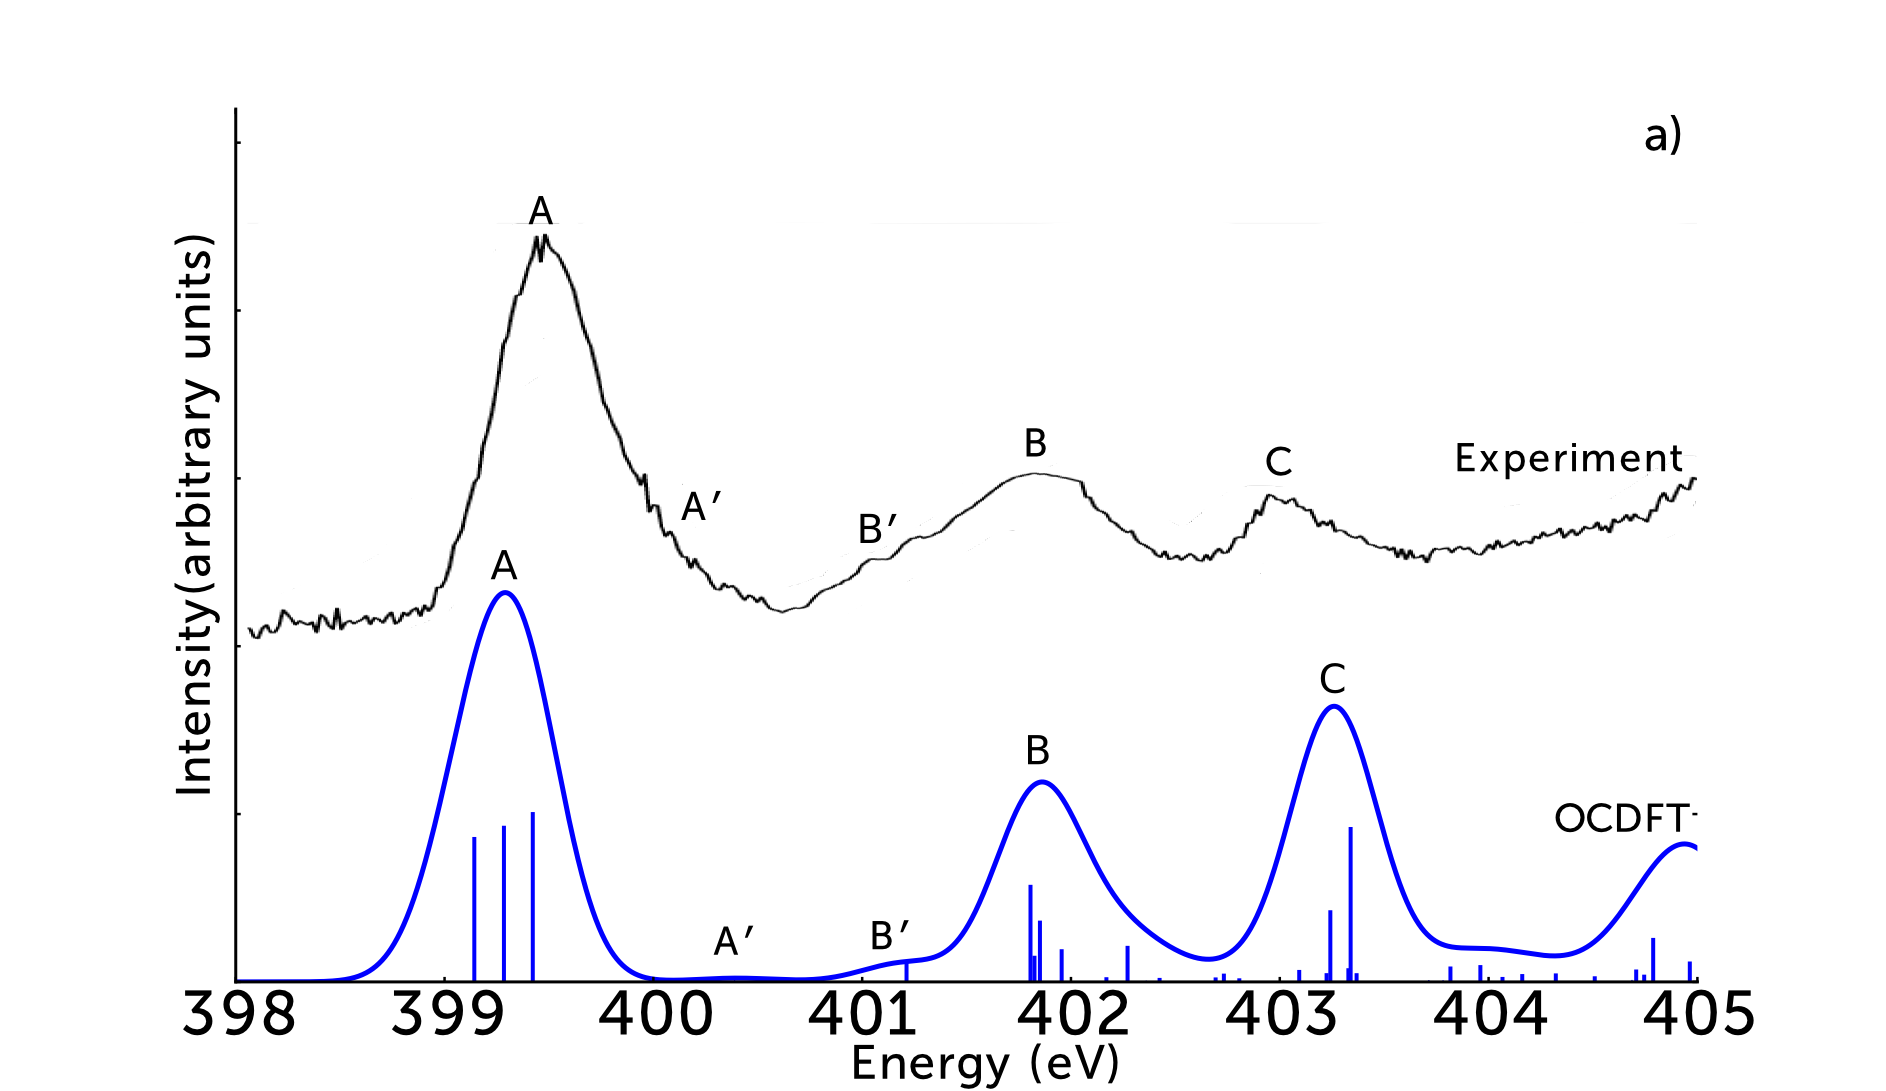
\includegraphics[scale=0.20]{AdenineNKexperiment.png} \\
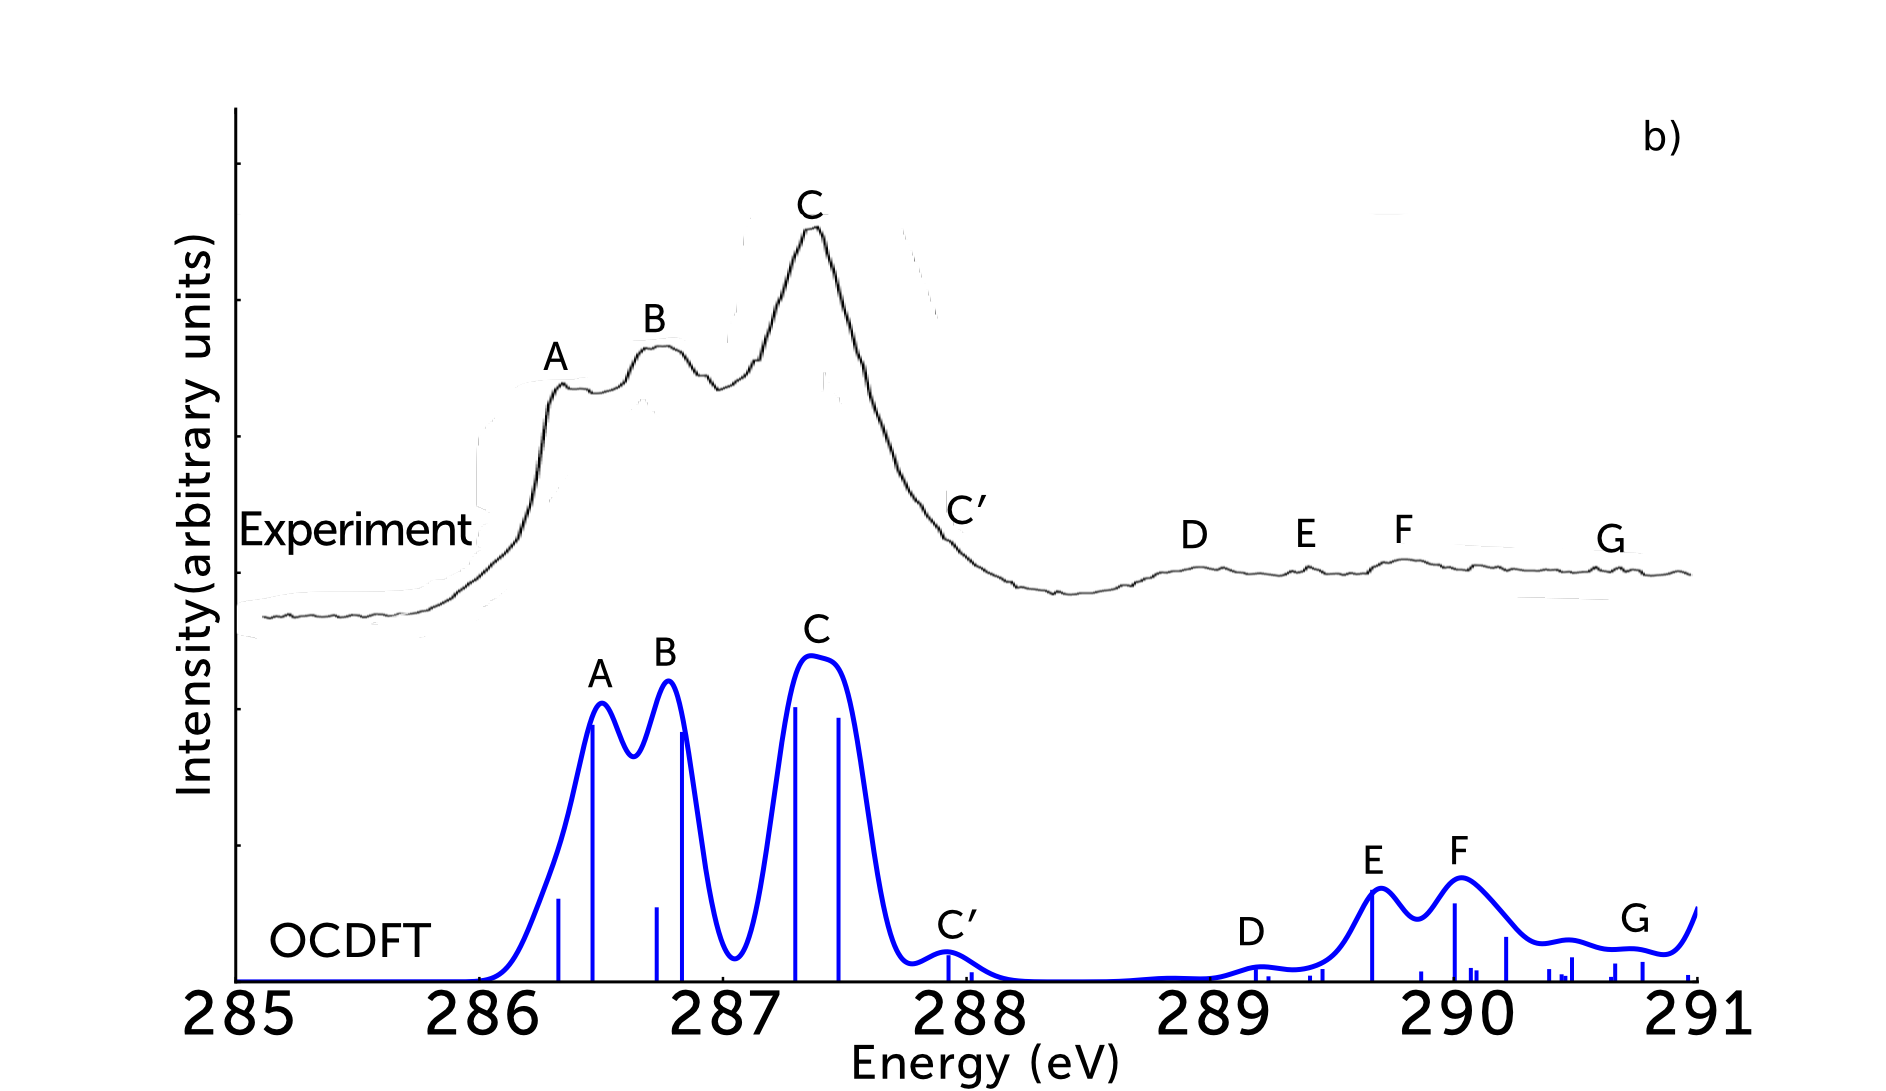
\includegraphics[scale=0.20]{AdenineCKexperiment.png}
\caption{Core excited states for adenine computed using B3LYP functional and def2-TZVP basis set. Spectra is composed of convoluted Gaussians with a FWHM of 0.2 eVs of the (a) nitrogen K-edge and (b) carbon K-edge.}
\label{figure:Adenine}
\end{figure}
 \begin{table}
 \centering
    \begin{tabular}{c@{\hskip 0.22in}c@{\hskip 0.22in}c@{\hskip 0.52in}c@{\hskip 0.22in}c@{\hskip 0.22in}c}
     \hline
     \hline
   \multicolumn{3}{c}{OCDFT} &\multicolumn{2}{c}{Experiment} \\
   \hline
   Assignment & $\omega_{fi}$ & f$_{rel}$ & Peak &  $\omega_{fi}$   \\
   \hline
 Assignment(71) & 399.14 & 0.852 \\
 Assignment(61) & 399.28 & 0.918 \\
 Assignment(81) & 399.42 & 1.000 \\
 Assignment(82) & 399.69 & 0.001 \\
 Assignment(72) & 400.39 & 0.022 \\
 Assignment(62) & 401.21 & 0.111 \\
 Assignment(41) & 401.81 & 0.567 \\
 Assignment(63) & 401.83 & 0.144 \\
 Assignment(51) & 401.85 & 0.353 \\
 Assignment(73) & 401.96 & 0.183 \\
 Assignment(84) & 402.17 & 0.016 \\
 Assignment(52) & 402.27 & 0.203 \\
 Assignment(74) & 402.36 & 0.004 \\
 Assignment(64) & 402.42 & 0.012 \\
 Assignment(83) & 402.69 & 0.015 \\
 Assignment(75) & 402.73 & 0.037 \\
 Assignment(65) & 402.81 & 0.009 \\
 Assignment(85) & 403.09 & 0.059 \\
 Assignment(76) & 403.22 & 0.033 \\
 Assignment(86) & 403.22 & 0.040 \\
 Assignment(43) & 403.24 & 0.415 \\
 Assignment(42) & 403.24 & 0.141 \\
 Assignment(66) & 403.33 & 0.070 \\
 Assignment(54) & 403.34 & 0.911 \\
 Assignment(87) & 403.37 & 0.040 \\
 Assignment(67) & 403.71 & 0.008 \\
 Assignment(77) & 403.78 & 0.006 \\
 Assignment(88) & 403.82 & 0.080 \\
 Assignment(44) & 403.96 & 0.088 \\
 Assignment(78) & 404.07 & 0.018 \\
 Assignment(79) & 404.16 & 0.035 \\
 Assignment(89) & 404.16 & 0.004 \\
 Assignment(55) & 404.32 & 0.039 \\
 Assignment(68) & 404.51 & 0.022 \\
 Assignment(53) & 404.69 & 0.008 \\
 Assignment(69) & 404.71 & 0.062 \\
 Assignment(90) & 404.75 & 0.031 \\
 Assignment(80) & 404.79 & 0.250 \\
 Assignment(56) & 404.96 & 0.110 \\
 Assignment(70) & 405.02 & 0.478 \\
 Assignment(57) & 405.26 & 0.048 \\
 Assignment(45) & 405.46 & 0.153 \\
 Assignment(46) & 405.62 & 0.073 \\
 Assignment(47) & 405.82 & 0.063 \\
 Assignment(58) & 406.14 & 0.167 \\
 Assignment(59) & 406.18 & 0.078 \\
 Assignment(60) & 406.69 & 0.080 \\
 Assignment(48) & 406.89 & 0.182 \\
 Assignment(50) & 407.02 & 0.156 \\
 Assignment(49) & 407.71 & 0.737 \\
    \end{tabular}
      \caption{Calculated and experimental thymine core excitation energies in eV are shown in the table. All excitations originate from the 1s orbital on the specified atom. \\
  $^{\ddagger}$Experimental value for this transition is inconclusive, value shown here was calculated using ADC(2)}
  \label{figure:MOs}
  \end{table}
   \begin{table}
 \centering
     \begin{tabular}{c@{\hskip 0.22in}c@{\hskip 0.22in}c@{\hskip 0.52in}c@{\hskip 0.22in}c@{\hskip 0.22in}c}
     \hline
     \hline
   \multicolumn{3}{c}{OCDFT} &\multicolumn{2}{c}{Experiment} \\
   \hline
   Assignment & $\omega_{fi}$ & f$_{rel}$ & Peak &  $\omega_{fi}$   \\
   \hline
 Assignment(81) & 286.32 & 0.298 \\
 Assignment(71) & 286.46 & 0.935 \\
 Assignment(82) & 286.73 & 0.266 \\
 Assignment(51) & 286.83 & 0.909 \\
 Assignment(41) & 287.30 & 1.000 \\
 Assignment(61) & 287.47 & 0.961 \\
 Assignment(62) & 287.87 & 0.001 \\
 Assignment(83) & 287.93 & 0.090 \\
 Assignment(72) & 288.02 & 0.028 \\
 Assignment(42) & 288.79 & 0.009 \\
 Assignment(84) & 288.88 & 0.006 \\
 Assignment(52) & 288.99 & 0.000 \\
 Assignment(85) & 289.19 & 0.039 \\
 Assignment(63) & 289.24 & 0.013 \\
 Assignment(73) & 289.41 & 0.016 \\
 Assignment(53) & 289.46 & 0.040 \\
 Assignment(54) & 289.66 & 0.330 \\
 Assignment(86) & 289.87 & 0.031 \\
 Assignment(74) & 290.00 & 0.281 \\
 Assignment(64) & 290.07 & 0.044 \\
 Assignment(43) & 290.09 & 0.035 \\
 Assignment(75) & 290.21 & 0.158 \\
 Assignment(87) & 290.39 & 0.040 \\
 Assignment(88) & 290.44 & 0.021 \\
 Assignment(76) & 290.46 & 0.015 \\
 Assignment(55) & 290.49 & 0.083 \\
 Assignment(65) & 290.65 & 0.011 \\
 Assignment(44) & 290.66 & 0.060 \\
 Assignment(56) & 290.77 & 0.066 \\
 Assignment(77) & 290.96 & 0.018 \\
 Assignment(89) & 291.05 & 0.248 \\
 Assignment(66) & 291.09 & 0.060 \\
 Assignment(45) & 291.14 & 0.054 \\
 Assignment(90) & 291.17 & 0.141 \\
 Assignment(57) & 291.42 & 0.003 \\
 Assignment(46) & 291.67 & 0.057 \\
 Assignment(67) & 291.68 & 0.125 \\
 Assignment(78) & 291.68 & 0.031 \\
 Assignment(79) & 291.90 & 0.026 \\
 Assignment(68) & 292.07 & 0.127 \\
 Assignment(47) & 292.14 & 0.051 \\
 Assignment(69) & 292.17 & 0.077 \\
 Assignment(48) & 292.41 & 0.021 \\
 Assignment(59) & 292.42 & 0.166 \\
 Assignment(80) & 292.59 & 0.018 \\
 Assignment(49) & 292.59 & 0.003 \\
 Assignment(60) & 292.70 & 0.235 \\
 Assignment(70) & 292.79 & 0.194 \\
 Assignment(58) & 292.84 & 0.105 \\
 Assignment(50) & 293.23 & 0.143 \\
     \end{tabular}
      \caption{Calculated and experimental thymine core excitation energies in eV are shown in the table. All excitations originate from the 1s orbital on the specified atom. \\
  $^{\ddagger}$Experimental value for this transition is inconclusive, value shown here was calculated using ADC(2)}
  \label{figure:MOs}
  \end{table}
\noindent The computed oxygen K-edge shown in Figure \ref{figure:Thymine}a is in good agreement with the experimental peaks. The two most dominant features of this spectra are excitations from the respective O 1s orbitals, to $\pi^*$ particle orbitals. The MCHP algorithm is able to reproduce these features well. The energy region above 534 eV is dominated by Rydberg transitions and mixed valence/Rydberg states and therefore is outside the scope of the current study. The most prominent feature of the experimental N K-edge shown in Figure \ref{figure:Thymine}b is the large peak near 403 eVs. This peak is a mix of valence and Rydberg excitations from the N$_3$ 1s and N$_4$ 1s orbitals, however because of the projective nature of the algorithm we are unable to calculate these states at this time. Peak C at 401.6 eVs is in excellent agreement with the experimental peak maximum around 401.7 eVs. The N 1s excitation manifold is complex, the experimental spectra is cluttered with multiple transitions within a small region. This makes it difficult to clarify exactly which experimental peak that D corresponds to, but we can compare our value to the same transition calculated using ADC(2) (See table in Figure \ref{figure:MOs} for details). Figure \ref{figure:Thymine}c shows that the computed C K-edge is in excellent agreement with experimental spectra. All of the prominent features of this spectra are excitations from C 1s orbitals to the $\pi^*$ particle orbitals. The computed line intensities are very similar to the experimental spectra giving us great confidence in the ability of OCDFT to compute the oscillator strengths of core-valence excited states.
Figure \ref{figure:Adenine} displays the nitrogen and carbon K-edges of adenine computed with OCDFT. Peak A, the most prominent feature of the spectra, contains contributions from three of the nitrogen atoms located on the ring system. Since peak A is composed entirely of valence excitations from unique 1s core orbitals, this is the best glimpse at the accuracy of OCDFT when it is able to calculate all peak contributions. The peak of the Gaussian formed by all contributions to the peak is centered around 399.3 eV, very close to the experimental peak centered at 399.5 eV. The relative line intensity, when compared to peaks B and C, is almost identical to the relative intensity seen in the experimental spectra. Peak B is largely a shoulder feature of peak C, and this relationship is captured perfectly in our theoretical spectra. The experimental peak at 403 eV is composed of Rydberg excitations from N$_3$ and N$_4$, outside the scope of the MCHP algorithm. The carbon K-edge is also in good agreement, once again we see a spectra whose main features can be captured without considering the Rydberg states. The three main peaks between 286 eV and 288 eV are well represented by OCDFT. The line intensity of peak F is replicated well, although the intensities of peaks D and E differ slightly from experiment. \\
\section{Conclusions}
Orthogonality constrained density functional theory represents a new frontier in simulating excited states using density functional methods. Many of the efforts in this field have centered around developing new functionals in order to compensate for the shortcomings of the standard GGA functionals by varying the amount of hartree-fock exchange and other parameters present in the functional. Previous studies done using time dependent density functional methods have all concluded that the 20-25\% hartree-fock exchange present in many standard hybrid functionals is not sufficient enough to describe core-excited states using TDDFT. However, here we show that standard functionals perform well with OCDFT at computing core-excited states due to the local nature of the integrals present in the excitation energy expression that allow for a better description of core-valence excitations. We have proven this by benchmarking OCDFT over a range of first and second row core excitations using standard pure and hybrid functionals. OCDFT showed no significant dependence on the amount of HF exchange, producing similar results across different functionals with varying fractions of HF exchange. OCDFT was also performed well across both the first and second row of the periodic table, only losing approximately 1.0 eV of accuracy when moving to the second row of the periodic table. Also outperforming TDDFT by ~11.1 eV when calculating first row core excitations, and by ~30.0 eV when calculating second row core excitations. We also calculate the nitrogen, oxygen, and carbon K-edges of thymine and adenine to show that OCDFT produces acceptable spectral profiles without the aid of an arbitrary energy shift.
\\ \\ 
Currently the biggest shortcoming of OCDFT is the limitations of the projective method to solving the Kohn--Sham equations. However this can be remedied by augmenting the code to allow for multiple projections from core orbitals. Once this is implemented, it should be possible to reproduce the complete NEXAS spectral profile of a system, this work is currently underway. Another area for improvement is to develop analytic energy gradients for OCDFT. This will allow us to study more complex systems and move beyond studying excited states and effectively study other molecular properties more throughly. We hope to present these extensions of this work in the near future.
\footnotesize{
\bibliography{OCDFT.bib} %your .bib file
\bibliographystyle{rsc} %the RSC's .bst file
}

\end{document}
